\newpage 
\part{Lecture Stochastic Processes}
\newpage



\chapter{Conditional expectation}
	\marginpar{\textcolor{red}{Lecture 1}}


Some people say advanced probability theory is measure theory plus conditioning. While elementary conditioning on events with positive probability is not a big deal this chapter covers conditioning on $\sigma$-algebras and random variables, topics which are central in statistics and probability theory. We will discuss several constructions
\begin{itemize}
	\item $\E[X|\mathcal F]$ - used in probability theory and mathematical finance for martingales,
	\item $\E[X|Y]$ and $\E[X|Y=y]$ - mostly used in statistics for regression,
	\item $\mathbb P(X\in A| Y)$ and $\mathbb P(X\in A\,|\, Y=y)$ - used to define a Markov process in probability theory.
\end{itemize}
One can already guess why many students struggle with conditional expectation. Similar objects appear in different contexts with different interpretations. On top, a bit like for the classical expectation, conditional expectation has concrete formulas for discrete and absolutely continuous random variables but has an abstract theoretical definition in the general case. 
%\section{Conditional Expectation}


%There are essentially two approaches towards conditional expectation. The first is of axiomatic nature, conditional expectation is defined through two measure theoretic axioms and then motivation is given by examples. The second is to first explain ideas in the discrete case and then derive the abstract axiom which is then used as a definition for the general case. We will follow the second approach, starting with a slightly lengthy discussion of "{}information"{} in probability.
\section{A hopefully gentle introduction}\label{sec:gentle}

	The main point in applications of conditional expectation is about information that is usually modelled using $\sigma$-algebras and measurability. In conditional expectation we will try to approximate random variables with other random variables that carry less "{}information"{} - which might already sound familiar from regression in statistics. For this sake, let $X$ be a real-valued random variable on a probability space $(\Omega, \mathcal A,\mathbb P)$. Recall from the very beginning of Stochastik 1 (Discussion \ref{N1}) the modelling idea of a measurable space in probability. The entire "{}knowledge of some abstract universe"{} is encoded in $\Omega$, $\omega$ refers to one particular instance of randomness in the universe, for instance some atomic collision. The $\sigma$-algebra $\mathcal A$ contains as sets the events in the universe which occurrence can be observed (e.g. an apple is falling down a tree). So far we fixed such "{}information"{} and considered observations of real values using the concept of random variables. The concept of "{}information"{} behind the random variable did not play a major role so far as computing expectations, variances, etc. only depends on the distribution function. We will now try to get a better feeling for "{}information"{} by comparing different $\sigma$-algebras and by discussing the "{}information"{} given by random variables.\smallskip
	
	To keep things simple suppose $X$ is a discrete random variable taking values $a_1,...,a_N\in\R$. So far we only think about the values of $X$, but we know more. We also know the events on which $X$ takes its values, namely $A_k:=\{\omega \in\Omega: X(\omega)=a_k\}\in \mathcal A$. In terms of information this is a partition of $\Omega$ (i.e. $\Omega=\cupdot_{k=1}^N A_k$) into the observable events that can be distinguished through the different outcomes of $X$.  Note that from this point of view the values of $X$ are irrelevant, they only need to be different. 
		\begin{luebung}
			For $A_1, ..., A_N\in \mathcal A$ describe explicitly the smallest $\sigma$-algebra containing all these events. If the $A_k$ are the events on that a discrete random variable takes its values, then this is nothing but $\sigma(X)$, the $\sigma$-algebra generated by $X$ defined in \ref{Kat}.
	\end{luebung}	
	Now suppose a second discrete random variable $Y$ is given. How should we compare the "{}information"{} given by $X$ and $Y$? How should we formalise that $Y$ carries more "{}information"{} than $X$? It seems quite plausible to say that $Y$ contains more "{}information"{} than $X$ if the outcomes of the random variable $X$ can be derived from the outcomes of the random variable $Y$. In more formal words, if the partition of $\Omega$ in "{}information"{} given by $Y$ is finer (see the picture) than the partition given by $X$. 
	 
\begin{figure}[h]
\begin{center}
\scalebox{0.6}{
\begin{tikzpicture}[rotate=15,transform shape]
  \node[ellipse,draw=black,fill=gray,fill opacity=0.4,minimum height=100pt,minimum width=200pt] (e) at (0,0) {};
  \node[rotate=-15] (O) at ($(e.-60) + (0.3,-0.3)$){};
  \draw[thick,draw=red] (0,0) -- (e.-150) coordinate (e1);
  \draw[thick,draw=red] (0,0) -- ($(e.-30)!.29!(e.-210)$) coordinate (e2);
  \draw[thick,draw=red] (0,0) -- (e.-210) coordinate (e3);
  \draw[thick,draw=red] (e.0)-- ($(e.0)!0.36!(e.180)$) coordinate (e4);
  \draw[thick,draw=orange] (e.60) -- (e.-60) ;
  \end{tikzpicture}
  }
  \vspace{-3mm}
  \caption*{Two partitions of $\Omega$ into two yellow or five red sets}
 \end{center}
\end{figure}
	 Formulated in terms of $\sigma$-algebras the notion of more information for random variables is nothing else but saying $\sigma(X)\subseteq \sigma(Y)$. A good example to keep in mind is the random variable $Y$ that measures some temperature in tenth of a degree celsius and the random variable $X$ that measures the same temperature only in degrees.
	 \begin{luebung}
	 	Draw a picture of the partitions of $\Omega$ for the simple temperature example. What are $\sigma(X)$ and $\sigma(Y)$? Make sure you understand why $\sigma(X)\subseteq \sigma(Y)$ holds.
	 \end{luebung}	
	 
	 
%\vspace{-4mm}
%	\begin{figure}[h]
%	\begin{center}
%		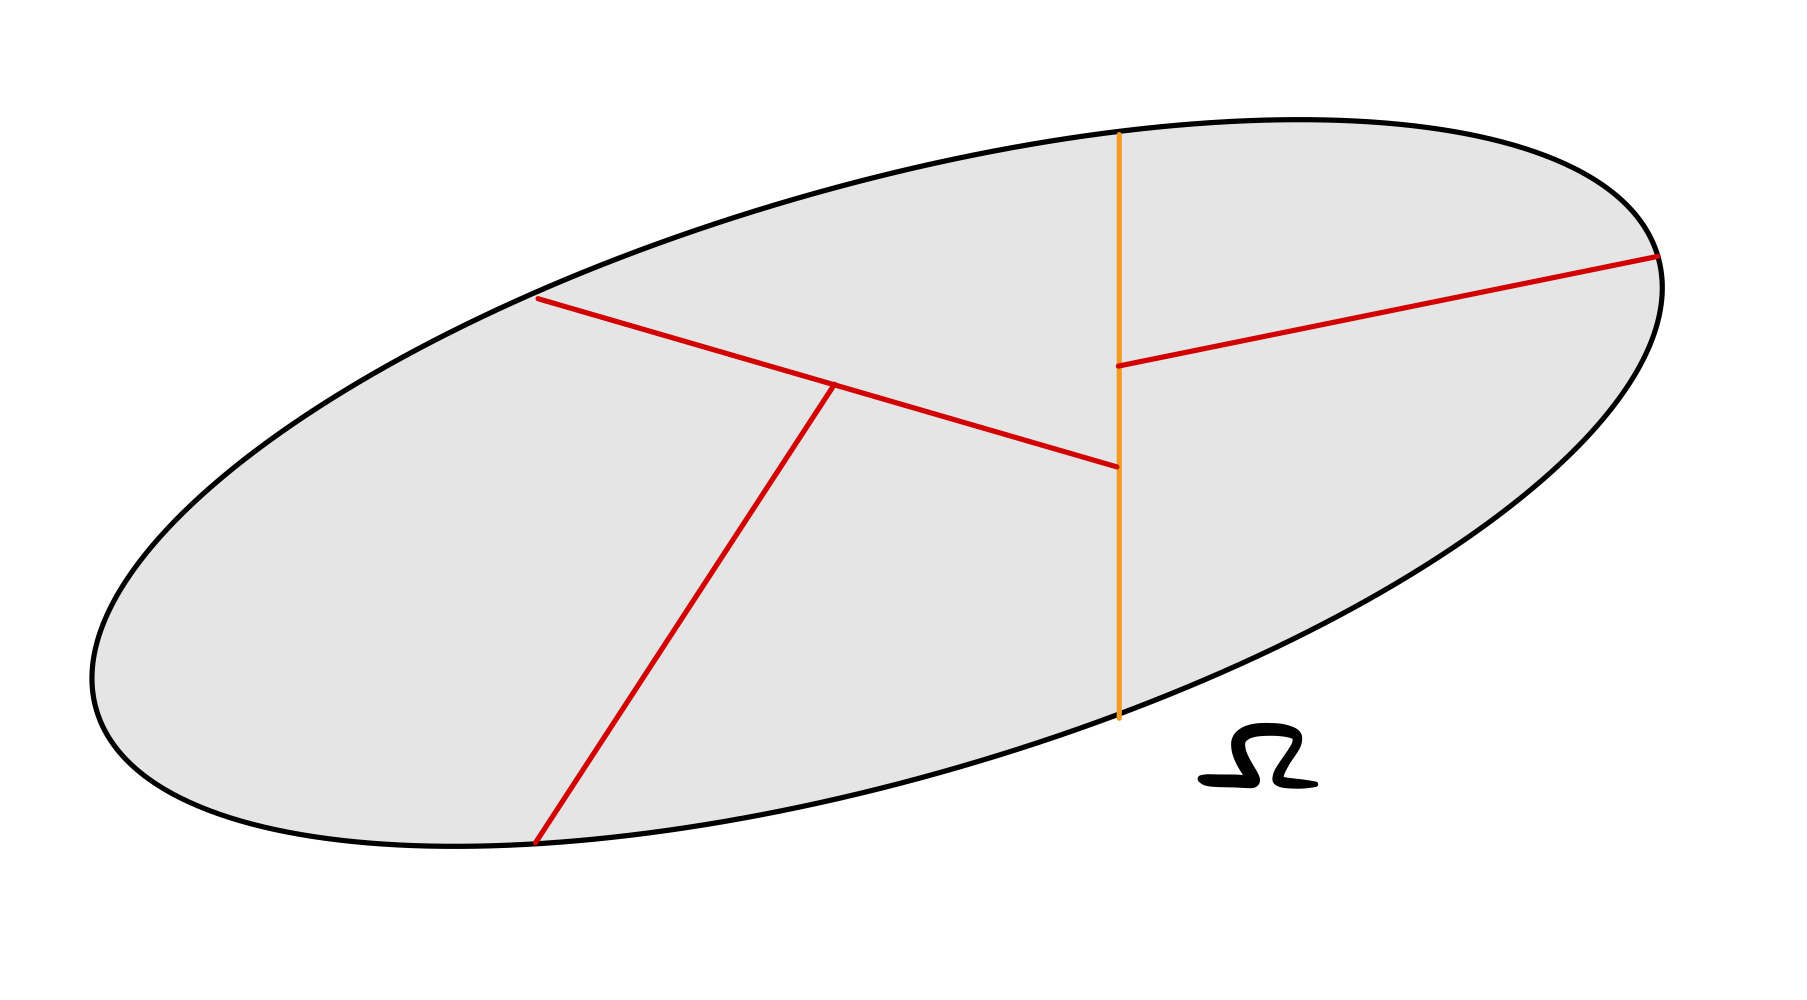
\includegraphics[scale=0.1]{CD0.jpeg}
%	\end{center}
%	\vspace{-1cm}
%	\caption*{Two partitions of $\Omega$, by two yellow or five red sets}
%	\end{figure}
	In mathematics it is important to chose examples which are not too simple and not too complicated in order to understand definitions. The best example to understand the concept of information of $\sigma$-algebras is probably the sequence of $\sigma$-algebras induced by a sequence of random variables. 
\begin{example}	
	Suppose $X_1,X_2,...$ is a sequence of random variables on $(\Omega, \mathcal A, \mathbb P)$, which we will later call a stochastic process. Then define
	\begin{align*}
		\mathcal F_n:=	\sigma(X_1,...,X_n):=\{ X_k^{-1}(B) : k\leq n,B\in \mathcal B(\R^n)\},\quad \text{ for }n\in\N.
	\end{align*}	
	It is clear from the definition that the sequence of $\sigma$-algebras $\mathcal F_n$ is increasing in the sense that $\mathcal F_n\subseteq \mathcal F_{n+1}$, thus, carries more and more "{}information"{}. Increasing sequences of $\sigma$-algebras will later-on be called filtrations. Let us assume, all $X_n$ are discrete random variables taking values in $\Z$ and check what "{}information"{} is carried by $\mathcal F_n$? Since everything is discrete we can write down all preimages to obtain simple generators of the $\sigma$-algebras:
		\begin{align*}
		\mathcal F_n
		&=\sigma(\{ \{X_1 \in A_1, ..., X_n \in A_n \} : A_i\subseteq \Z \})\\
		&=\sigma(\{\{X_1=i_1,..., X_n=i_n\}: i_k\in \Z \}).
	\end{align*}	
	Formulated in words, $\mathcal F_n$ is generated by events under which the process follows a given path, or, in other words, $\mathcal F_n$ contains all events which occurrence can be decided by looking at the first $n$ steps of the stochastic process. Increasing the time of the process thus leads to a larger set of observable events, thus, to more "{}information"{}. As an example let us check that the event "{}$0$ was hit before time $n$"{} belongs to $\mathcal F_n$ (but not to $\mathcal F_k$ for $k<n$):
	\begin{align*}
		&\quad \{0\text{ was hit before time }n\}\\
		&=\{0\text{ was hit at time }1\}\cup...\cup \{0\text{ was hit at time }n\}\\
		&= \bigcup_{i_2,i_3,...,i_n\in \Z} \{X_1= 0, X_2=i_2,..., X_n=i_n\}
		 \cup...\cup \bigcup_{i_1,...,i_{n-1} \in\Z} \{X_1= i_1, ..., X_{n-1}=i_{n-1},X_n=0 \}\\
		&\in \mathcal F_n.
	\end{align*}
	It is a good exercise to think of some other event and try to check that they belong (or do not belong) to the information of the first $n$ steps $\mathcal F_n$.
	
\end{example}
	These first thoughts comparing finitely many events break down immediately when the random variables fail to be discrete. To generalise we can only work with the generated $\sigma$-algebras
	\begin{align*}
		\sigma(X)=\{ X^{-1}(B): B\in \mathcal B(\R)\}.
	\end{align*}
	Recall that $\sigma(X)$ is the smallest $\sigma$-algebra on $\Omega$ so that $X$ is measurable. If $X$ is discrete $\sigma(X)$ only contains the events $\{X=a_k\}$ and their unions and complements. The discussion above suggests to say that $Y$ carries more "{}information"{} than $X$ if $\sigma(X)\subseteq \sigma (Y)$. To go even further, we can remove the concept of a random variable from the discussion. Similarly as above, we extend the idea of "{}information"{} to general $\sigma$-algebras by saying an $\sigma$-algebra $\mathcal F$ carries the "{}information"{} of its events. If $\mathcal B$ and $\mathcal F$ are $\sigma$-algebras on $\Omega$ we say that $\mathcal B$ carries more "{}information"{} than $\mathcal F$ if $\mathcal F\subseteq \mathcal B$. Recalling the motivation of $\sigma$-algebras comprising the observable events of the universe that makes perfect sense.\smallskip
	
The information that two $\sigma$-algebras are generated by random variables is extremely valuable. It allows to formalise the concept of more/less information in the following way:
\begin{lsatzwichtig}
\begin{lemma}[Doob's factorisation lemma]
		Let $X, Y$ two random variables on $(\Omega, \mathcal A, \mathbb P)$. If $X$ is measurable with respect to $\sigma(Y)$, i.e. $\sigma(X)\subseteq \sigma(Y)$, then there is a Borel-measurable mapping $h:\R\to\R$ such that $X=h(Y)$.
	\end{lemma}
\end{lsatzwichtig}
	\begin{proof}[Proof]
		Exercise. First understand the statement if $Y$ (and thus $X$) is discrete, $h$ can easily be written down. You can see that your $h$ can be defined arbitrarily for values that $Y$ does not take. Then approximate $Y$ using a sequence of step functions as in Theorem \ref{k} and use the appearing sequence of mappings $h_n$ to define $h$ as their pointwise limit.
	\end{proof}	
	\begin{lwarnhinweis}
		The function $h$ is not unique! Changing $h$ on values that $Y$ does not take will not change $h(Y)$.
	\end{lwarnhinweis}

	 A random variable $X$ carrying less "{}information"{} than another random variable $Y$ is thus only a transformation of $Y$ and as such, not more complicated than $Y$. In the example of measuring temperatures with different thermometers, depending on the thermometers, the mapping $h$ might just erase the decimals. The factorisation $h$ simplifies the more fine information $\{Y=5,0\}$, ..., $\{Y=5,9\}$ into one $\{X=5\}$.  The reverse statement does not hold. In the setting of the theorem there will usually not be a mapping $g$ such that $Y=g(X)$, the random variable $X$ cannot explain the random variable $Y$ without further information, think of measuring the temperature!\smallskip
	
	 Now suppose we are in a situation in which the factorisation does not apply but we would still like to express $Y$ as good as we can through $X$. Imagine $Y$ is a feature vector that we are interested in but we can only observe some simpler feature vector $X$ of which we believe $X$ should be able to explain $Y$ reasonably well. In statistics or machine learning you might have seen the idea of regressing $Y$ on $X$ in different contexts, such as finding a neural network functions such that $Y\approx f(X)$. In the following we discuss the measure theoretic version of this problem which is motivated from the factorisation lemma. If $Y$ cannot be written as $h(X)$ then at least we aim at finding a measurable function $h$ such that $Y\approx h(X)$ with a rigorously defined meaning of $\approx$. If we formalise $\approx$ through the $L^2$-distance of random variables, then - at least for square-integrable random variables - we can solve the minimisation problem using so-called conditional expectations. \smallskip
	 
	 
Before motivating conditional expectations through best approximation let us recall an elementary but important fact of expectations that should be familiar from Stochastik 2:
	
	
	
%	generated by a random vector $X=(X_1,...,X_n)$ or, equivalently, by random variables $X_1,...,X_n$. In probability we say that $\sigma(X)$ contains the "{}information"{} we get from $X$. But what does this mean? A real-valued random variable is a mapping that returns real values for each $\omega$ from the usually unknown source of all randomness $\Omega$. This is everything that potentially happens in the "{}universe"{}, but we are only able observe if the events $A\in \mathcal A$ happen or not. We can for instance not observe all collisions of atoms but we can observe certain more macroscopic events such as a tree falling or not. For the random variable $X$ the generated $\sigma$-algebra contains precisely those events that determine the outcome of $X$. For a better understanding let us consider the case of a discrete random variable taking values $a_1,...,a_N$ for which we have the simpler expression
%	\begin{align*}
%		\sigma(X)=\{ \cup_{i\in I} \{X= a_i\}: I\subseteq \{1,...,N\}\}=\sigma(\{\{X=a_i\}: i\in \{1,...,N\}\}).
%	\end{align*}
%	If $X$ only takes two values, the generated $\sigma$-algebra is $\{\Omega, \emptyset, \{X=a_1\}, \{X=a_2\}\}.$ The more complex (more possible outcomes) $X$ becomes, the larger the generated $\sigma$-algebra becomes. Similarly, if $X_1,...,X_n$ are all discrete random variables the generated $\sigma$-algebra 
	
%ANDERSRUM AUFSCHREIBEN. Erst erklaeren, was info sein sollte, dann beispiel, dann die erzeugte sigma-algebra erklaeren.	
\begin{lstep}
Given a random variable $X$, how would we best approximate $X$ by a constant value? As an instructive example, without any further thought, how would we approximate a $\mathcal N(\mu,\sigma^2)$-random variable best with a constant random variable? Of course using $Y\equiv \mu$, what else? To get the intuition straight let's check the $L^2$-approximation property of the expectation by solving
\begin{align*}
	\min_{\theta\in\R} \E[(X-\theta)^2].
\end{align*}
Expanding the square and minimising the quadratic function the solution to this simple approximation problem gives $\theta^*=\E[X]$. 
\end{lstep}
Here is a simple visualisation that will be useful for conditional expectations in a bit:
%	\begin{figure}[h]
%	\begin{center}
%		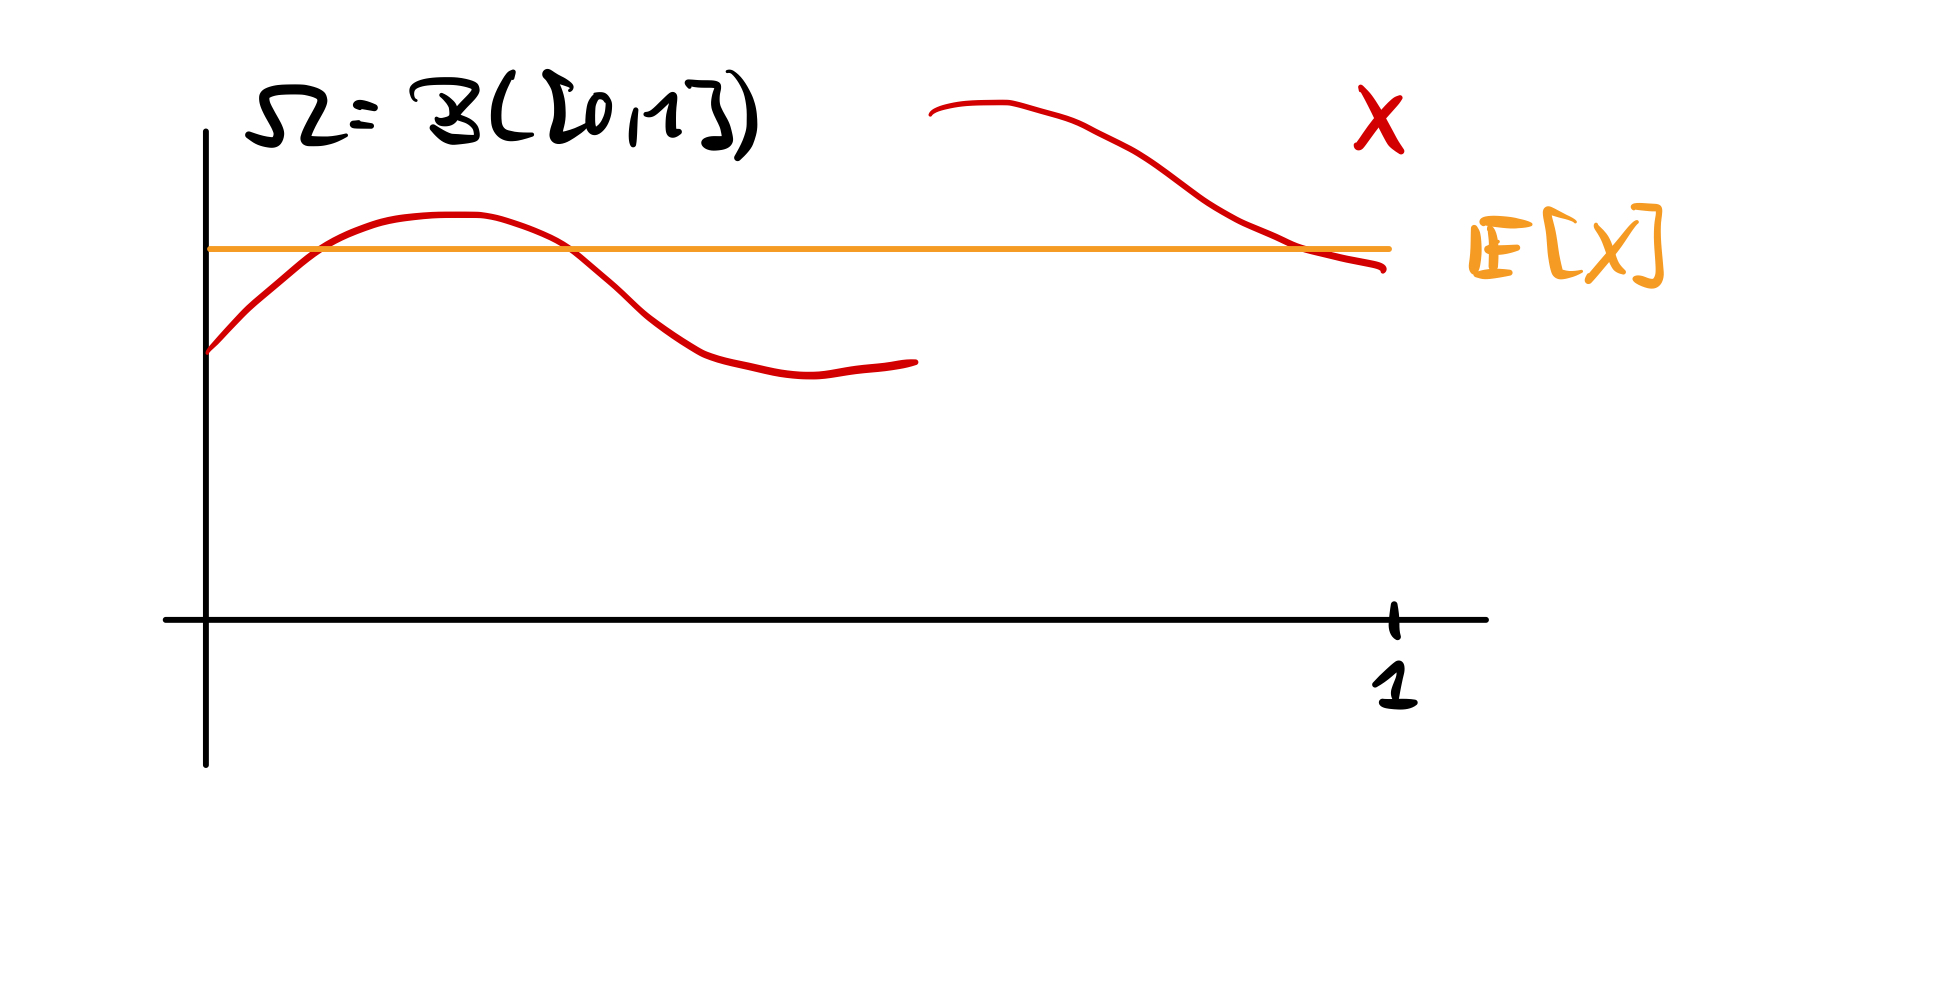
\includegraphics[scale=0.1]{CE4.jpeg}
%	\end{center}
%	\vspace{-1.3cm}
%	\caption*{Illustration of $L^2$-approximation of $X$ through the expectation}
%	\end{figure}

\begin{figure}[h]
\begin{center}
\scalebox{0.8}{
\begin{tikzpicture}
    \node at (2,3.3) (nodeO) {$\Omega=[0,1], \mathcal{A} = \mathcal{B}([0,1])$};
    \node[orange] at (6.2,2) (nodeA) {$Y=\mathbb{E}[X ]$};
    \node[red] (nodeX) at ($(nodeA.south)+(-0.6,-0.1)$) {X};
    \node (t1) at (5,-.3) {1};
    \draw (5,-.1) -- (5,.1);
    %AXIS Y
    \draw (0,0) -- ++(90:3cm);
    %AXIS X 
    \draw (0,0) --++(0:5.5cm);

    \draw[thick,orange](0,2) -- (5,2);
    \draw[thick,red]  (0,1.5) .. controls (1.2,3.2)  and (1.5,1.3) .. (3.2,1.6);
    \draw[thick,red]  (3.2,2.75) .. controls (3.8,3) and (4.5,1.8)  .. (5,1.9);
  \end{tikzpicture}
  }
  \vspace{-3mm}
  \caption*{Illustration of best $L^2$-approximation of $X$ through the expectation}
\end{center}
\end{figure}
\begin{lwarnhinweis}
Warning: People say "{}the best estimation of a random variable without further information is the expectation"{} but this is only correct if we talk about minimisation of the $L^2$-distance. Minimising $\E[|X-\theta|]$ leads to the median, not the expectation! \smallskip
\end{lwarnhinweis}

Let us now return to the approximation of random variables through random variables carrying less information, using the $L^2$-distance. Suppose we have a random variable $X$ on $(\Omega, \mathcal A, \mathbb P)$ and a discrete $\sigma$-algebra $\mathcal F\subsetneq \sigma(X)$, let's say $\mathcal F=\sigma(B_1,...,B_K)$ or, alternatively, $\mathcal F=\sigma(Y)$ for some random variable of the form $Y=\sum_{l=1}^K b_l \mathbf 1_{B_l}$. Now assume  we would like to explain $X$ as good as we can using only the "{}information"{} from $\mathcal F$ (or alternatively from $Y$). It is not possible to write $X=h(Y)$ as all $\mathcal F$-measurable functions take the form
\begin{align*}
	h(Y)= \sum_{l=1}^K h(b_l) \mathbf 1_{B_l}
\end{align*}
so that $X=h(Y)$ would contradict $\mathcal F\subsetneq \sigma(X)$. Instead, we try to best approximate $X$ by all $\mathcal F$-measurable random variables $\sum_{l=1}^K \beta_l \mathbf 1_{B_l}$, again in the $L^2$-sense as this is the easiest for computations.



\begin{figure}[h]
\begin{center}
  \hspace{10mm}
\begin{tikzpicture}
  \node at (0.3,0.5+1) (sum) {$h(y) = \sum_{l=1}^K \beta_l \mathbf{1}_{B_l}(y)$};
  \draw (0,0) ellipse (2 and 1);

\foreach \x/\n/\h in {0.07/a/0.40,0.35/b/0.17,-0.69/c/0.15,-0.04/d/-0.28,-0.47/h/-0.22,0.47/i/-0.13,0.72/j/0.29,-0.71/k/-0.48,0.49/l/0.71,-0.10/n/-0.76,0.04/o/0.00}{
    \node (\n)[circle,inner sep=2.5pt] at (\x,\h){};
    \draw[darkgreen] (\n.north west)--(\n.south east)(\n.south west)--(\n.north east);
}
  \draw[-stealth,darkgreen,thick] (sum) -- (0.2,0.7);
  \node[circle,inner sep=1.3pt,fill=black] (X) at (2.5,0.6) {} ;
  \node (x) at ($(X.east)+(0.3,-0)$) {$X$};
  \node (R) at (1.8,0.2) [circle,fill,inner sep=1.3pt,red]{};
  \node at (1.5,0) [red]{?};
  \draw[-stealth,red,thick] ($(X)+(-0.1,-0.05)$) -- (R);

  %%GUIDELINE
  %\draw[grey!50] (R) -- ++(0.7,0);
%  \draw[grey!50] (X) -- ++(0,-0.4);
  %%
  \end{tikzpicture}
  \vspace{-2mm}
 \caption*{Approximating X best from the set of all $\mathcal{F}$-measurable random variables}
\end{center}
\end{figure}
Let us solve the minimisation problem
\begin{align*}
	\min_{Z\, \mathcal F\text{-measurable}}\E[(X-Z)^2]
\end{align*}
without thinking much by just rewriting
\begin{align*}
	 \min_{Z\, \mathcal F\text{-measurable}}\E[(X-Z)^2]
	&=\min_{\beta_1,...,\beta_K} \E\Big[\Big(X-\sum_{l=1}^K \beta_l \mathbf 1_{B_l}\Big)^2\Big]\\
	&=\min_{\beta_1,...,\beta_K} \E\Big[\Big(\sum_{l=1}^K(X- \beta_l )\mathbf 1_{B_l}\Big)^2\Big]\\
	\overset{B_i\cap B_j=\emptyset}&{=}\min_{\beta_1,...,\beta_K} \sum_{l=1}^K\E\big[(X- \beta_l )^2 \mathbf 1_{B_l}\big]
\end{align*}
Minimising the right-hand side over the vector $\beta$ gives 
\begin{align*}
	\beta=\Big(\frac{\E[X \mathbf 1_{B_1}]}{\mathbb P(B_1)},...,\frac{\E[X \mathbf 1_{B_K}]}{\mathbb P(B_K)}\Big).
\end{align*} 
Introducing the notation $\E[X| A]:= \frac{\E[X \mathbf 1_{A}]}{\mathbb P(A)}$ we get the following solution of the $L^2$-approximation problem:
\begin{align}\label{cd1}
	Z^*=\sum_{l=1}^K \E[X| B_l] \mathbf 1_{B_l}.
\end{align} 
We will denote this random variable by $\E[X| \mathcal F]$ and call it the conditional expectation of $X$ given $\mathcal F$. $\E[X|\mathcal F]$ is the most we can say about $X$ (in the $L^2$-sense) with the information given by $\mathcal F$.
%	\begin{figure}[h]
%	\begin{center}
%		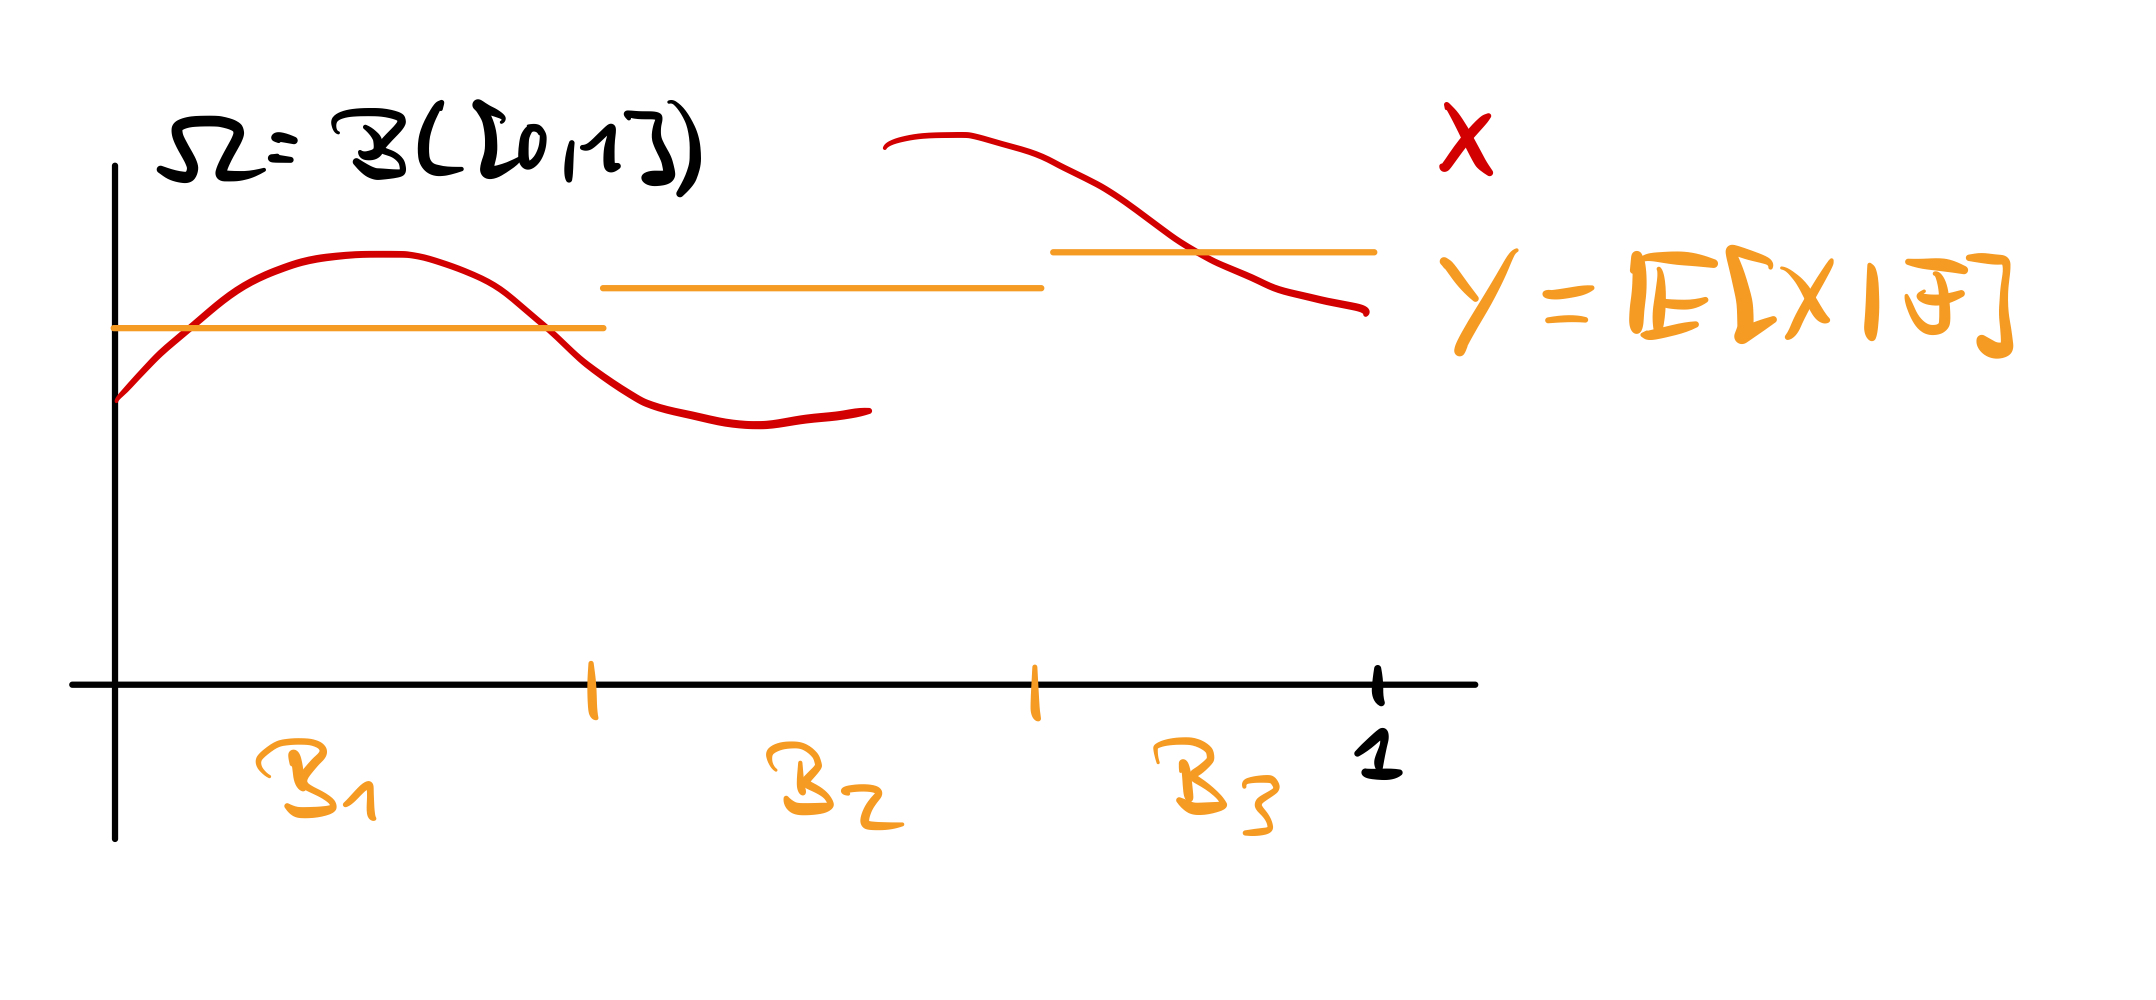
\includegraphics[scale=0.1]{CE2.jpeg}
%	\end{center}
%	\vspace{-1cm}
%	\caption*{Illustration of best $L^2$-approximation of $X$ through $\mathcal F$-measurable random variables}
%	\end{figure}

\begin{figure}[h]
\begin{center}
\scalebox{0.8}{
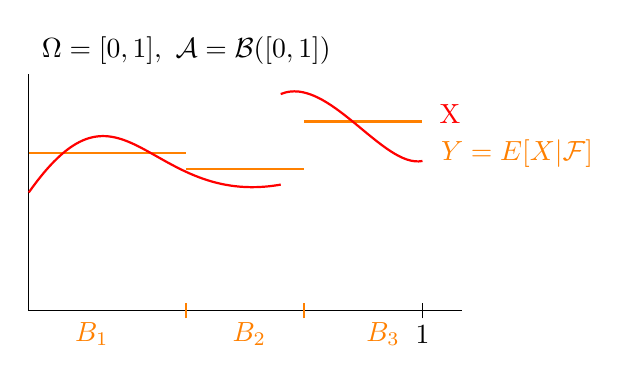
\begin{tikzpicture}
    \node (t1) at (5,-.3) {1};
    \draw (5,-.1) -- (5,.1);
    \draw ([yshift=-0.2]t1) -- ([yshift=0.2]t1) ;
    %AXIS Y
    \draw (0,0) -- ++(90:3cm);
    %AXIS X 
    \draw (0,0) --++(0:5.5cm);

    \node at (2,3.3) (nodeO) {$\Omega=[0,1], \ \mathcal{A} = \mathcal{B}([0,1])$};
    \node[orange] at (6.2,2) (nodeA) {$Y=\mathbb{E}[X| \mathcal{F}]$};
    \node[red] (nodeX) at (5.35,2.5) {X};
    \node[orange] at (0.8,-0.3) (B1) {$B_{1}$};
    \node[orange] at (2.8,-0.3) (B2) {$B_{2}$};
    \node[orange] at (4.5,-0.3) (B3) {$B_{3}$};
    
    %Y CURVE
    \draw[thick,orange](0,2) -- (2,2);
    \draw[thick,orange](2,1.8) -- (3.5,1.8);
    \draw[thick,orange](3.5,2.4) -- (5,2.4);

    \draw[thick, orange] (2,-0.1) -- (2,0.1);
    \draw[thick, orange] (3.5,-0.1) -- (3.5,0.1);
    %X CURVE
    \draw[thick,red] plot [smooth]  (0,1.5) .. controls (1.2,3.2)  and (1.5,1.3) .. (3.2,1.6);
    \draw[thick,red] plot [smooth]  (3.2,2.75) .. controls (3.8,3) and (4.5,1.8)  .. (5,1.9);
  \end{tikzpicture}
  }
  \vspace{-3mm}
    \caption*{Best $L^2$-approximation in the light of approximation through simple functions}
  \end{center}
\end{figure}
The computation above did not shed much light on what is going on. Could we have guessed the formula \eqref{cd1} without computations? For that sake let us recall the interpretation of elementary conditional probability measures $\mathbb P(\cdot \,|\, B):=\frac{\mathbb P(\cdot\, \cap B)}{\mathbb P(B)}$. The original random experiment is restricted to a subexperiment on $B$. All knowledge from $\Omega\backslash B$ is forgotten for the subexperiment, the relative probabilities of events $A\subseteq B$ remain unchanged by normalising all events with the same factor $\mathbb P(B)$. If $X$ was a random variable on $\Omega$ then the restriction to $ B$ is a random variable on the restriction $(B, \mathcal A_{|  B}, \mathbb P_{| B})$ with $\E_{| B}[X]=\E[X| B]$. We also call $\E_{|B}$ elementary conditional expectation. With this interpretation of elementary conditioning in mind formula \eqref{cd1} is nothing but $K$-times elementary $L^2$-approximation with constants for the $K$ restricted random variables $X_{|B}$. 
%	\begin{figure}[h]
%	\begin{center}
%		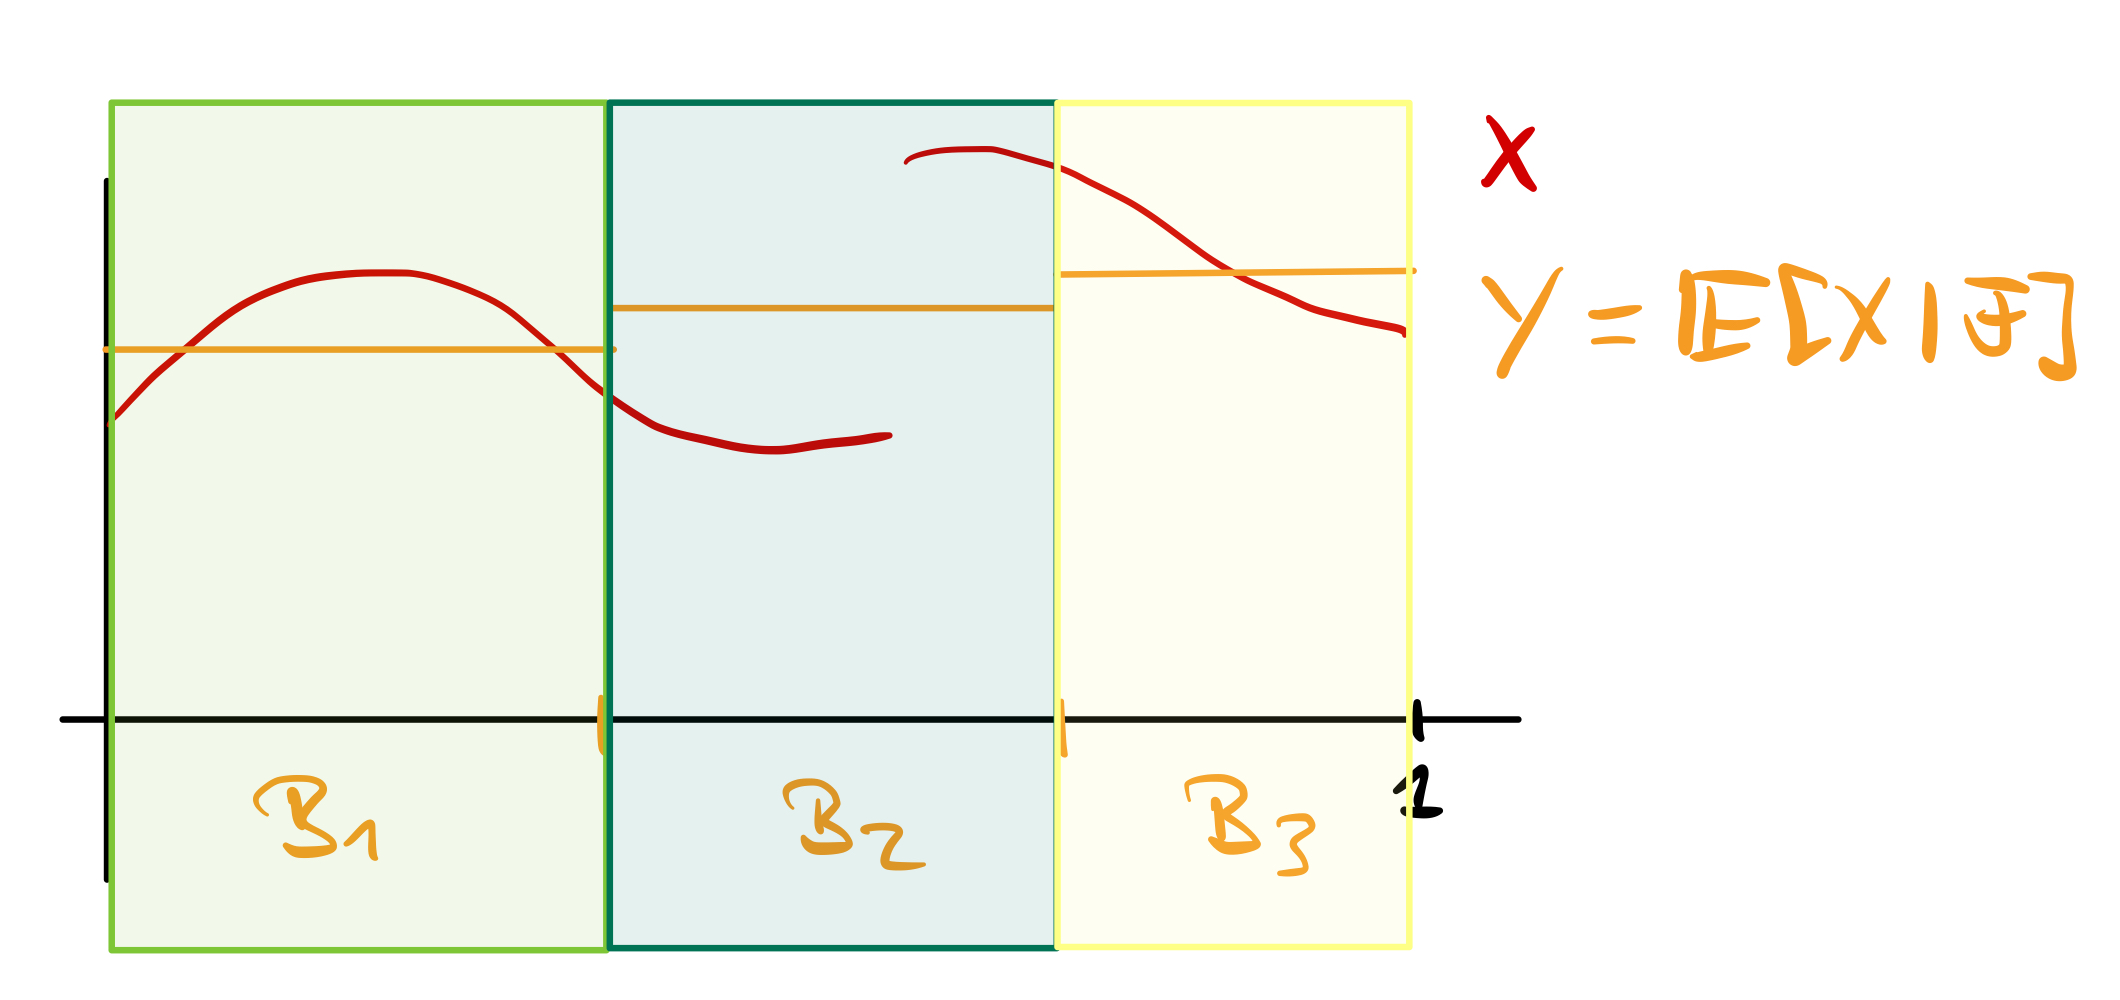
\includegraphics[scale=0.1]{CE5.jpeg}
%	\end{center}
%	\vspace{-0.7cm}
%	\caption*{Illustration of $L^2$-approximation through constant $L^2$-approximations of subexperiments}
%	\end{figure}

\begin{figure}[h]
\begin{center}
\scalebox{0.8}{
\begin{tikzpicture}
    \node (t1) at (5,-.3) {1};
    \draw (5,-.1) -- (5,.1);
    \draw ([yshift=-0.2]t1) -- ([yshift=0.2]t1) ;
    %AXIS Y
    \draw (0,0) -- ++(90:3cm);
    %AXIS X 
    \draw (0,0) --++(0:5.5cm);

    \node[orange] at (6.2,2) (nodeA) {$Y=\mathbb{E}[X| \mathcal{F}]$};
    \node[red] (nodeX) at (5.35,2.5) {X};

    \node[orange] at (0.8,-0.3) (B1) {$B_{1}$};
    \node[orange] at (2.8,-0.3) (B2) {$B_{2}$};
    \node[orange] at (4.5,-0.3) (B3) {$B_{3}$};

    \draw[thick, orange] (3.5,-0.1) -- (3.5,0.1);
    \draw[thick, orange] (2,-0.1) -- (2,0.1);

    \draw[thick,orange](0,2) -- (2,2);
    \draw[thick,orange](2,1.8) -- (3.5,1.8);
    \draw[thick,orange](3.5,2.4) -- (5,2.4);

    %X CURVE
    \draw[thick,red] plot [smooth]  (0,1.5) .. controls (1.2,3.2)  and (1.5,1.3) .. (3.2,1.6);
    \draw[thick,red] plot [smooth]  (3.2,2.75) .. controls (3.8,3) and (4.5,1.8)  .. (5,1.9);

    \draw[ultra thick,draw=darkgreen,fill=green,opacity=0.2]
      (0,-0.5) rectangle (2,3.2);

    \draw[ultra thick,draw=darkgreen,fill=darkgreen,opacity=0.2]
      (2,-0.5) rectangle (3.5,3.2);

    \draw[ultra thick,draw=darkgreen,fill=yellow,opacity=0.2]
      (3.5,-0.5) rectangle (5,3.2);
  \end{tikzpicture}
  }
 \caption*{Best $L^2$-approximation in the light of constant approximation on subexperiments}

  \end{center}
\end{figure}

Writing these thoughts formally by introducing $1=\sum_{l=1}^K \mathbf 1_{B_l}$ for the splitting the experiment into the $K$ subexperiments gives 
\begin{align*}
	\E[(X-Y)^2]&=\E\Big[\Big(\sum_{l=1}^K (X-\beta_l) \mathbf 1_{B_l} \Big)^2\Big]
	=\sum_{l=1}^K \E[(X-\beta)^2 \mathbf 1_{B_l}]=\sum_{l=1}^K \E_{|B_l}[(X-\beta_l)^2]\mathbb P(B_l).
\end{align*}
Best $L^2$-approximating all $K$ subexperiments by constants gives the same solution $\beta$ that we have found above by direct computation. The advantage is our better understanding of the appearing factors as elementary conditional expectations $\E_{|B_l}[X]$.\smallskip

In many textbooks on probability theory the motivation of conditional expectations is less formal, taking for granted that the best approximation of a random variable without extra information is the expectation. The intuitive reasoning is that the conditional expectation is the expectation given prior knowledge. Even though the statement "{}given"{} is very imprecise (the true formulation is $L^2$-minimisation as above) it works intuitively quite well. 
\begin{example}
	Suppose $X$ denotes a dice taking values $1,...,6$ with probabilities $\frac 1 6$. What is our best guess for $X$ if we know that the dice is even (or odd)? Keeping the $L^2$-minimisation property of expectations in mind we should  compute the expectations of the conditional experiments, the dice conditioned on being even (or odd). Intuitively, this is $4$ in the even and $3$ in the odd case. Denoting by $\mathcal F=\{\Omega, \emptyset, \{1,3,5\},\{2,4,6\}\}$ the additional information we have this is nothing but a sketch of the rigorous formula $$\E[X|\mathcal F]= \E[X|X \in \{1,3,5\} ] \mathbf 1_{X\in \{1,3,5\}}+\E[X|X\in \{2,4,6\}]\mathbf 1_{X\in \{2,4,5\}}$$ from above. Plug-in the definition of the elementary conditional expectations to check they give $3$ and $4$! 
\end{example}


There is a major challenge remaining. How do we generalise the above reasoning to general random variables and general $\sigma$-algebras if we cannot easily compute with finite sums of indicators? We follow the axiomatic approach of Kolmogorov in which the conditional expectations $\E[X|\mathcal F]$ and $\E[X|Y]$ are  defined through the two axiomatic properties
\begin{itemize}
	\item $\E[X|\mathcal F]$ is $\mathcal F$-measurable,
	\item $\E\big[\E[X|\mathcal F\big] \mathbf 1_A]=\E[X \mathbf 1_A]$ holds for all $A\in \mathcal F$.
\end{itemize}
Before discussing for general random variables how these properties define a reasonable object let us check that our discrete conditional expectation satisfies these properties. The measurability is a matter of our approach, we only minimised the distance over $\mathcal F$-measurable random variables. The more strange second property can be checked through the following quick computation. Let us first assume $A$ is equal to precisely one of the $B_l$, thus, disjoint from all the others:
\begin{align*}
	\E\big[ \E[X|\mathcal F] \mathbf 1_A\big]&=\E\Big[\sum_{l=1}^K \E[X|B_l]\mathbf 1_{B_l} \mathbf 1_A\Big]
	=\E\big[  \E[X|A] \mathbf 1_A\big]
	=\E[X|A] \E[\mathbf 1_A]
	\overset{\text{def}}{=} \E[X \mathbf 1_A].
%	&=\E\Big[  \E\Big[\sum_{n=1}^N \alpha_n \mathbf 1_{A_n}  \Big|A\Big] \mathbf 1_A\Big]\\
%	\overset{Lin., def.}&{=} \sum_{n=1}^N \E\Big[ \alpha_n \frac{\mathbb P(A_n\cap A)}{\mathbb P(A)}\mathbf 1_A\Big]\\
%	\overset{Lin.}&{=}\sum_{n=1}^N \alpha_n \mathbb P(A_n\cap A)\\
%	&=\E\Big[\sum_{n=1}^N \alpha_n \mathbf 1_{A_n }\mathbf 1_A\Big]
\end{align*}
Since all $A\in \mathcal F$ can be written as finite union of the $B_k$ the general claim follows from linearity.\smallskip

The magic of conditional expectation is that the preceding two properties are all we need for a powerful definition of general conditional expectation with amazing consequences!


\section{The axiomatic approach of Kolmogorov}


We shall now turn to a general setup, dropping the assumption of discrete random variables and finite $\sigma$-algebras. We will reverse the story and start with an axiomatic definition of conditional expectation from which we then derive abstract existence and identify key properties (such as $L^2$-error minimization) that reflect the motivation given before. 

\begin{ldefwichtig}
\begin{deff}\label{deff_condexp}
	Let $(\Omega, \mathcal A, \mathbb P)$ a probability space, $X\in \mathcal L^1(\Omega, \mathcal A, \mathbb P)$, and $\mathcal F$ a sub-$\sigma$-Algebra of $\mathcal A$. Then a random variable $Z$  on $(\Omega, \mathcal A, \mathbb P)$ is called the \textbf{conditional expectation of $X$ given $\mathcal F$} if
	\begin{itemize}
		\item $Z$ is $\mathcal F$-measurable,
		\item $\mathbb E[Z \mathbf 1_A]=\mathbb E[X \mathbf 1_A]$ for all $A\in \mathcal F$.
	\end{itemize}
	If such a random variable $Z$ exists, then we write $Z=E[X|\mathcal F]$. If $\mathcal F=\sigma(Y)$ for a  random variable $Y$ then we write $Z=\E[X|Y]$ and call $Z$ the \textbf{conditional expectation of $X$ give $Y$}.
\end{deff}
\end{ldefwichtig}
Choosing $A=\Omega$ in the second condition it is clear that the integrability assumption on $X$ cannot be avoided. In contrast to the section before we cannot use $L^2$-distances, second moments are not assumed to be finite. It is important to note that the very definition of $\E[X|\mathcal F]$ shows that conditional expectation is not defined uniquely. This is caused by the second property as expectations do not change if random variables are changed on zero sets. Any other $\mathcal F$-measurable random variable $\bar Z$ that equals $Z$ almost surely will automatically satisfy the second condition.
\begin{ldef}
\begin{deff}
	Suppose $Z$ and $\bar Z$ are random variables on a probability space $(\Omega, \mathcal A, \mathbb P)$. We call $\bar Z$ a \textbf{version} of $Z$ if $\mathbb P(Z=\bar Z)=1$.
\end{deff}
\end{ldef}
We will see later that it can be useful to choose particularly versions of the conditional expectation that satisfies additional measurability properties.

\begin{lsatzwichtig}
\begin{theorem}\label{existenceCE}
	Let $X$ an integrable random variable on $(\Omega, \mathcal A, \mathbb P)$ and $\mathcal F$ a sub-$\sigma$-algebra of $\mathcal A$. Then the conditional expectation $\E[X|\mathcal F]$ exists and is almost surely unique, i.e. two random variables satisfying the two defining properties are versions of each other.
\end{theorem}
\end{lsatzwichtig}
\begin{proof}[Proof]
	\textbf{Uniqueness:} Suppose $Z$ and $\bar Z$ are random variables fulfilling the two defining properties of Definition \ref{deff_condexp} and let $A=\{\bar Z<Z\}\in\mathcal{F}.$ Using the second property of conditional expectation, it holds that 
	$$0=\E[\mathbf{1}_AZ]-\E[\mathbf{1}_A\bar{Z}]=\E[(Z-\bar{Z})\mathbf{1}_A]\ge0.$$ It follows that $\mathbf{1}_A(Z-\bar{Z})=0$ almost surely. Similarly, it holds that $\mathds{1}_{A^c}(Z-\bar{Z})=0$ almost surely. Taking the unions of the nullsets gives $Z=\bar Z$ almost surely.\smallskip
	
	\textbf{Existence:} To prove the existence we use the Radon-Nykodyn from functional analysis. The theorem states that a $\sigma$-finite measure $\nu$ has a density with respect to another $\sigma$-finite measure $\mu$ if and only if $\nu\ll \mu$. Here we use the absolutely continuity notion $\mu\ll \mu$ if every zero set for $\mu$ is also a zero set for $\nu$. The interested reader is referred any book containing enough Functional Analysis \footnote{For instance P. Billingsley, 1995, "{}Probability and Measure"{} (3rd edition), Wiley, pp. 419–427}. Now let 
	\begin{align}\label{eq_05}
		Q^+:\cF\to[0,1],A\mapsto\E[X^+\mathbf{1}_A]\quad\text{ and }\quad Q^-:\cF\to[0,1],A\mapsto\E[X^-\mathbf{1}_A],
	\end{align}
	which are both $\sigma$-finite measures on $\mathcal F$ with $Q^+\ll \mathbb P$ and $Q^-\ll \mathbb P$. Hence, there are $\mathcal{F}$-measurable densities $Z^+,Z^-$ with $$Q^+(A)=\int_A Z^+\dint\mathds{P}\quad \text{ and }\quad Q^-(A)=\int_A Z^-\dint\mathds{P}$$ for all $A\in\cA$. Let $Z:=Z^+-Z^-$, then $Y$ is $\cF$ measurable and 
	\begin{align*}
		\E[\mathbf{1}_AZ]&=\E[\mathbf{1}_AZ^+]-\E[\mathbf{1}_AZ^-]\\
		&=\int_AZ^+\dint\mathds{P}-\int_AZ^+\dint\mathds{P}\\
		&\overset{\eqref{eq_05}}=Q^+(A)-Q^-(A)\\
		&=\E[\mathbf{1}_AX^+]-\E[\mathbf{1}_AX^-]\\
		&=E[\mathbf{1}_AX].
	\end{align*}
	Therefore, the random variable $Z$ fullfills the properties of the conditional expectation of $X$ given $\cF$.
\end{proof}
	\marginpar{\textcolor{red}{Lecture 2}}


Just as for typical expectations we continue with a set of properties fulfilled by the conditional expectation. Some properties look familiar to old properties of expectations, but always keep in mind: conditional expectations are random variables! 

\begin{lsatzwichtig}
\begin{theorem}[Standard properties of conditional expectation]\label{cond_properties}
	Let $X,Y\in\cL^1(\Omega,\cA,\mathbb{P})$, $\lambda\in \R$, and $\cG\subseteq\cF\subseteq\cA$ sub-$\sigma$-Algebras. Then the following properties hold:
		\begin{enumerate}[label=(\roman*)]
			\item $\E\big[\E[X\,|\,\mathcal F]\big]=\E[X]$ and  $\E[1\,|\, \mathcal F]=1$ a.s.
			\item $\mathds{E}[\,\lambda X+Y \,|\, \mathcal{F}\,]=\lambda\mathds{E}[\, X \, | \, \mathcal{F}\, ]+\mathds{E}[Y \, | \, \mathcal{F}]$ a.s.
			\item $X \geq Y$ a.s. $\Rightarrow \mathds{E}[X\, |\, \mathcal{F}] \geq \mathds{E}[Y \,|\, \mathcal{F}]$ a.s.
			\item If $\mathds{E}[\lvert XY \rvert] < \infty$ and $Y$ is $\mathcal{F}$-measurable, then
				$$\mathds{E}[XY\,|\,\cF] = Y\mathds{E}[X\,|\,\cF]\:\:\text{a.s.}\quad \text{ and }\quad \mathds{E}[Y\,|\,\cF]=Y\:\:\text{a.s.}$$
			\item $\mathds{E}\big[\mathds{E}[X\,|\,\cF]\,\big|\,\cG\big] = \mathds{E}\big[\mathds{E}[X\,|\,\cG]\,\big|\,\cF\big]=\mathds{E}[X\,|\,\cG]$ a.s.
			\item $\big\lvert\mathds{E}[X\,|\,\cF]\big\rvert \leq \mathds{E}\big[\lvert X \rvert\,\big|\,\cF\big]$ a.s.
			\item If $\sigma(X)$ and $\cF$ are independent, then $\mathbb E[X\,|\,\cF] = \mathbb E[X]$ a.s.
			\item If $\mathbb{P}(A)\in \{0,1\}$ for all $A \in \cF$, then $\mathbb E[X\,|\,\cF] = \mathbb E[X]$ a.s.
			\item If $\E[X|\mathcal F]$ is a.s. constant, then $\E[X|\mathcal F]=\E[X]$ a.s.
			\item If $\E[X\mathbf 1_A]=\E[Y\mathbf 1_A]$ for all $A\in \mathcal F$, then $\E[X|\mathcal F]=\E[Y|\mathcal F]$ a.s.
			\item Suppose $\lvert X_n \rvert \leq Y$ a.s. for $Y \in \cL^1(\Omega, \mathcal A, \mathbb P)$ and $\lim\limits_{n \to \infty}X_n = X$ a.s., then
				$$\lim\limits_{n \to \infty}{ \mathbb E[X_n\,|\,\cF]}=\mathbb E[X\,|\,\cF] \,\,\text{ a.s and in }L^1.$$ 
			\item Suppose $X_n\geq 0$ is an increasing sequence of random variables with $\lim_{n\to\infty} X_n=X$ a.s., then 
				$$\lim\limits_{n \to \infty}{ \mathbb E[X_n\,|\,\cF]}=\mathbb E[X\,|\,\cF] \,\,\text{ a.s}.$$ 			
				
	\end{enumerate}
\end{theorem}
\end{lsatzwichtig}
\begin{proof}[Proof]
	\begin{enumerate}[label=(\roman*)]
		\item Exercise
		\item The trick is always the same: If we intend to prove $\E[...|...]=Z$ a.s., we need to check for $Z$ the two defining properties of the claimed conditional expectation. Uniqueness of conditional expectations then implies that $Z$ is a version of the conditional expectation. Following once in detail this routine let us denote the righthand side by $Z$. Since $Z$ is a linear combination of two $\mathcal F$-measurable random variables, $Z$ is $\mathcal F$-measurable, which is the first condition of conditional expectation. For the expectation condition, with $A\in\mathcal F$, we obtain, using properties of the usual expectation (linearity and (ii) of Theorem \ref{S7}) and the second property of the conditional expectations $\E[X\,|\,\mathcal F]$, $\E[Y\,|\, \mathcal F]$,
			\begin{align*}
				\E[\mathbf 1_A Z F]&=\mathbb E[\mathbf{1}_A(\lambda\mathds{E}[\, X \, | \, \mathcal{F}\, ]+\mathds{E}[Y \, | \, \mathcal{F}])]\\
				&=\lambda\mathbb E[\mathbf{1}_A\mathbb E[X\,|\,\cF]]+\mathbb E[\mathbf{1}_A\mathbb E[Y\,|\,\cF]]\\
					&=\lambda\mathbb E[\mathbf{1}_A X]+\mathbb E[\mathbf{1}_A Y]\\
					&=\mathbb E[\mathbf 1_A (\lambda X+Y)].
			\end{align*}
			Hence, $Z$ satisfies the defining conditions of $\E[\lambda X+Y\, |\, \mathcal F]$.
		\item \label{ii} Lemma \ref{me} tells us that $A:=\lbrace\mathbb E[X|\cF]<\mathbb E[Y|\cF]\rbrace\in \cF$. Using monotonicity of expectations and linearity of conditional expectations from (ii) gives
			$$0 \geq \mathbb E[\mathbf 1_A (\mathbb E[X\,|\,\cF]-\mathbb E[X\,|\,\cF])] =\mathbb E[\mathbf 1_A \mathbb E[X-Y\,|\,\cF]] = \mathbb E[\mathbf 1_A (X-Y)]\overset{\text{ass.}}{\geq} 0.$$ Since $\mathbf 1_A (\mathbb E[X\,|\,\cF]-\mathbb E[Y\,|\,\cF]) \leq 0$ by definition of $A$ we find $\mathbf 1_A (\mathbb E[X\,|\,\cF]-\mathbb E[Y\,|\,\cF]) = 0$ a.s. (Theorem \ref{S7}, (iii)) which gives $\mathbf 1_A = 0$ a.s. or, equivalently, $\mathbb E[X\,|\,\cF]\geq\mathbb E[Y\,|\,\cF]$ a.s.
		\item The proof works through discretisation and linearity. First assume $X,Y\geq 0$. Define $Y_n = \frac{1}{2^n} \cdot \lfloor 2^n \cdot Y \rfloor$ (draw a picture to undestand it!) so that almost surely $Y_n \nearrow Y$ and $$Y_n \mathbb E[X\,|\,\cF] \nearrow Y \mathbb E[X\,|\,\cF].$$ MCT for usual expectations implies $\lim \limits_{n \to \infty}\mathbb E[\mathbf 1_A Y_n \mathbb E[X\,|\,\cF]]=\mathbb E[\mathbf 1_A Y \mathbb E[X\,|\,\cF]]$ for $A\in\cF$. Now we compute the left-hand side:
			\begin{align*}
				\mathbb E\left[\mathbf 1_A Y_n \mathbb E[X\,|\,\cF]\right]&=\mathbb E\bigg[\mathbf 1_A \sum_{k=0}^\infty \frac{k}{2^n}\mathbf 1_{Y_n=\frac{k}{2^n}}\mathbb E[X\,|\,\cF]\bigg] \\
				\overset{\text{MCT}}&{=} \sum_{k=0}^\infty\mathbb E\bigg[\mathbf 1_A \frac{k}{2^n}\mathbf 1_{Y_n=\frac{k}{2^n}}\mathbb E[X\,|\,\cF]\bigg]\\
				&= \sum_{k=0}^\infty\mathbb E\bigg[\mathbf 1_A \frac{k}{2^n}\mathbf 1_{Y_n=\frac{k}{2^n}} X\bigg]\overset{\text{MCT}}{=}\mathbb E[\mathbf 1_A Y_n X]
			\end{align*}
			Again MCT yields $\mathbb E[\mathbf 1_A Y X]=\mathbb E[\mathbf 1_A Y \mathbb E[X\,|\,\cF]]$ which shows the expectation condition $$\mathbb E[Y X\,|\,\cF]=Y \mathbb E[X\,|\,\cF].$$ The $\mathcal F$-measurability of $Y\E[X|\mathcal F]$ follows from measurability of products.
			For the general case we proceed as usually, writing $X=X^+ - X^-$,$Y=Y^+ - Y^-$ and then using linearity from (ii). The second claim follows from (i) using $X=1$.
		\item Exercise
		\item The proof is exactly the same that we have already encountered for the classical expectation in Lemma \ref{properties}:
			\begin{align*}
				\big\lvert \mathbb E[X\,|\,\cF] \big\rvert &= \big\lvert \mathbb E[X^+\,|\,\cF]-\mathbb E[X^-\,|\,\cF]\big\rvert \\ 
				\overset{\Delta}&{\leq} \big \lvert \mathbb E[X^+\,|\,\cF] \big\rvert + \big\lvert \mathbb E[X^-\,|\,\cF] \big\rvert \\
				&= \mathbb E[X^+\,|\,\cF] + \mathbb E[X^-\,|\,\cF] \\
				&= \mathbb E[X^+ + X^-\,|\,\cF] \\
				&= \mathbb E\big[\lvert X \rvert \,\big|\,\cF\big]
			\end{align*}
		\item First recall that one (of several equivalent) ways to state the independence is to say that $X$ is independent of $\mathbf 1_A$ for all $A\in \mathcal F$. Using the factorisation of expectations of independent random variables gives
						\[	\mathbb E[\mathbf 1_A X] \overset{\text{ind.}}{=} \mathbb E[X]\mathbb E[\mathbf 1_A] \overset{\text{lin.}}{=} \mathbb E[\mathbb E[X]\mathbf 1_A] \]		
		for all $A\in \mathcal F$. Since additionally all constant random variables are $\mathcal F$-measurable, $\E[X]$ is a version of $\E[X\,|\, \mathcal F]$.

		\item The "trivial"{} $\sigma$-algebra $\cF$ is independent of all sub-$\sigma$-algebras $\cA$, in particular of $\sigma(X)$. Now use (vii).
		\item Suppose $\E[X|\mathcal F]=c$ almost surely. The defining property yields $\E[X\mathbf 1_A]=\E[ c\, \mathbf 1_A]=c\, \P(A)$ for all $A\in \mathcal F$. Now choose $A=\Omega$ and the claim follows.
		\item We show that $\E[Y|\mathcal F]$ satisfies the defining properties of $\E[X|\mathcal F]$ and then apply the uniqueness. Measurability follows from the measurability of conditional expectations, the expectation property as follows:
		\begin{align*}
			\E[X\mathbf 1_A]=\E[Y\mathbf 1_A]\overset{(i)}{=}\E\big[\E[Y\mathbf 1_A|\mathcal F]\big]\overset{(iv)}{=}\E\big[\E[Y|\mathcal F]\mathbf 1_A\big],\quad \forall A\in \cF.
		\end{align*}
		\item Define $Z_n = \sup\limits_{k\geq n}\lvert X_k - X \rvert$ so that $0\leq Z_n \leq 2Y$ and $Z_n \rightarrow 0,n \rightarrow \infty$. By usual DCT we find $\mathbb E[Z_n]\rightarrow 0$ for $n \rightarrow \infty$. The $L^1$-convergence can now be deduced as
				\begin{align*}
					\mathbb E\big[\lvert \mathbb E[X_n\,|\,\cF]-\mathbb E[X\,|\,\cF]\rvert\big]
					\overset{\Delta}{\leq} \mathbb E\big[\mathbb E[\lvert X_n - X \rvert \,|\,\cF]\big] = \mathbb E[\lvert X_n - X \rvert] \rightarrow 0,\quad n \rightarrow \infty
				\end{align*}
Next, towards the almost sure convergence. Since $Z_n$ is decreasing in $n$ the monotonicity implies that $\mathbb E[Z_n\,|\,\cF]$ is decreasing. Denote the limit by $M$. With Fatou we get $$0 \leq \mathbb E[M] \leq \liminf\limits_{n \rightarrow \infty}\mathbb E[\mathbb E[Z_n\,|\,\cF]]= \liminf\limits_{n \rightarrow \infty}\mathbb E[Z_n] = 0.$$ Hence, $M = 0$ a.s. Finally, we can conclude $$0\leq \lim_{n\to\infty} \lvert \mathbb E[X_n\,|\,\cF]-\mathbb E[X\,|\,\cF]\rvert \leq \lim_{n\to\infty} \mathbb E[Z_n\,|\,\cF] = M = 0.$$
	\item Using the monotonicity yields that $0\leq \E[X_n|\mathcal F]\leq \E[X_{n+1}|\mathcal F]\leq ...\leq \E[X|\mathcal F]$ so there is an almost sure limit $V:=\lim_{n\to\infty} \E[X_n|\mathcal F]$ and $V\leq \E[X|\mathcal F]$. Define $B=\{V<\E[X|\mathcal F]\}$, then
	\begin{align*}
		\E\big[ \E[X|\mathcal F] \mathbf 1_B\big]
		\overset{B\in \mathcal F}&=	\E[X \mathbf 1_B]\\
		\overset{\text{MCT}}&{=} \lim_{n\to\infty} \E[X_n \mathbf 1_B]\\
				\overset{(i)}&{=} \lim_{n\to\infty} \E\big[\E[X_n \mathbf 1_B|\mathcal F]\big]\\
		\overset{B\in \mathcal F}&=\lim_{n\to\infty} \E\big[\E[X_n |\mathcal F]\mathbf 1_B\big]\\
		\overset{\text{MCT}}&{=} \E[V\mathbf 1_B]\\
	\end{align*}
	But then $\P(B)$ must be $0$ as otherwise the equalities could not hold.	
	\end{enumerate}
\end{proof}
\begin{lsatz}
\begin{theorem}[Jensen's inequality for conditional expectation]
	Suppose $\varphi$ is convex with $X,\varphi (X) \in \mathcal L^1(\Omega,\cA,\mathds P)$, then
		\begin{align*}
			\varphi\big(\mathbb E[X\,|\,\cF]\big) \leq \mathbb E[\varphi(X)\,|\,\cF] \:\: \text{ a.s}.
		\end{align*}
\end{theorem}
\end{lsatz}
\begin{proof}[Proof]
			
	Let $E_\varphi=\lbrace (a,b)\in \mathbb{R}^2:\varphi(x)\geq ax+b,\forall x\rbrace$ the set of all subtangents. Then one (of many) ways to express the convexity is the expression
		\begin{align*}
			\varphi(x) = \sup\limits_{(a,b)\in E_\varphi}(ax+b) = \sup\limits_{(a,b)\in E_\varphi \cap \mathbb{Q}^2}(ax+b)
		\end{align*}



\begin{figure}[h]
\begin{center}

\scalebox{0.8} {
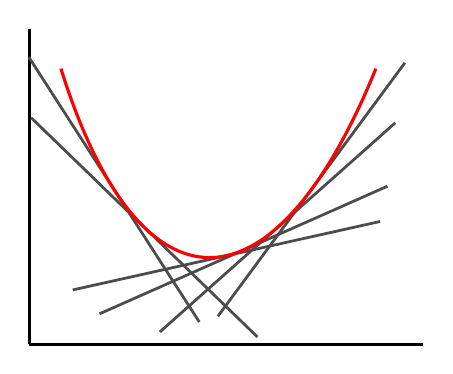
\begin{tikzpicture}
    %AXIS Y
    \draw[black,line width=0.4mm] (0.5,0) -- ++(90:4cm);
    %AXIS X 
    \draw[black,line width=0.4mm] (0.5,0) --++(0:5cm);
    % CURVE
    \begin{scope}[xshift=-1mm,yshift=-5mm]
    \path[thick,red] (1,4) .. controls (2,0.8) and (3.7,0.8) .. (5,4) 
      %TO MAKE NEW TANGENT LINE JUST COPY LINE BELOW AND CHANGE POS ,  xsep is length of line , 0.5 is min of curve 
      node[sloped,inner xsep =20mm,inner ysep=0,fill,pos=0.6,black!70]  {} 
      node[sloped,inner xsep =20mm,inner ysep=0,fill,pos=0.3,black!70]  {}
      node[sloped,inner xsep =20mm,inner ysep=0,fill,pos=0.7,black!70]  {}
      node[sloped,inner xsep =20mm,inner ysep=0,fill,pos=0.8,black!70]  {}
      node[sloped,inner xsep =20mm,inner ysep=0,fill,pos=0.55,black!70] {}
      node[sloped,inner xsep =20mm,inner ysep=0,fill,pos=0.2,black!70]  {} ;
    \draw[line width=0.4mm,red] (1,4) .. controls (2,0.8) and (3.7,0.8) .. (5,4);
    \end{scope}
  \end{tikzpicture}
  }
  \caption*{Representation of convex function through subtangents}
  \end{center}
\end{figure}

	Then,
		\begin{align*}
			\mathbb E[\varphi(X)\,|\,\cF] &= \mathbb E\Big[\sup\limits_{(a,b)\in E_\varphi \cap \mathbb{Q}^2}(aX+b)\,\Big|\,\cF\Big] \\
										\overset{\text{monotonicity}}&{\geq} \sup\limits_{(a,b)\in E_\varphi \cap \mathbb{Q}^2} \mathbb E[(aX+b)\,|\,\cF] \\ 
										\overset{\text{lin.}}&{=} \sup\limits_{(a,b)\in E_\varphi \cap \mathbb{Q}^2} \big(a \mathbb E[X\,|\,\cF]+b\big) \\
										&= \varphi\big(\mathbb E[X\,|\,\cF]\big).
		\end{align*}
		There is a very important point to make in this calculation. Applying the calculation rules result in a.s. statements for all applications of the rules. The chain of equalities and inequalities holds on the intersection of those events of probability one. Since also their intersection has probability one, the chain and the statement holds almost surely.
\end{proof}

We can now turn back towards our original interpretation of approximating random variables with random variables that carry less information. In general our approach to minimise $\E[(X-Y)^2]$ is not suitable as the expectation could be infinite. This is one of the reasons why in probability theory we tend to work with the abstract definition instead of an $L^2$-minimisation definition. Still, if we impose the extra assumption that $X$ is square-integrable we indeed have the $L^2$-minimisation property:
\begin{lsatz}
\begin{theorem}
	If $X$ is square-integrable, then $\mathbb E[X|\cF]$ is the orthogonal projection of $X$ to $\mathcal L^2(\Omega, \mathcal F, \P)$. Equivalently, the $L^2$-minimisation property holds:
	\begin{align*}
		\mathbb E[(X-Y)^2] \geq \mathbb E[(X-\mathbb E[X\,|\,\cF])^2],\quad \forall Y\in \mathcal L^2(\Omega, \mathcal F, \mathbb P),
	\end{align*}
	with equality if and only if $Y = \mathbb E[X|\cF]$.
\end{theorem}
\end{lsatz}
\begin{proof}[Proof]
	Let us recall from Functional Analysis the concept of an orthogonal projection. If $(H,\langle \cdot, \cdot\rangle)$ is a Hilbert space, $G$ a closed subspace and $P:H\to G$ a linear operator. Then $P$ is called an orthogonal projection if either
\begin{itemize}
	\item $\langle y, x-Px\rangle=0$ for all $y \in G$, or,
	\item $|| x-y||_{H}\geq || x-Px||_H$ for all $y\in G$.
\end{itemize}	
Both properties can be best understood in a picture.


\begin{figure}[h]
\begin{center}
\begin{tikzpicture}[rotate=15,transform shape]
  \draw[ultra thick, draw=black] (0,0) -- (4,0) ;
  \node[red] (xPx) at (1.3,1) {x-Px};
  \node[draw,circle,fill,inner sep=1.5pt] (Px) at (2,0) {};
  \node[black] (PxText) at ($(Px.south) +(-0,-0.2)$) {Px};
  \node[violet] (Y) at (2.7,0.2) {y};
  \draw[thick,red] (Px)-- ++(90:2cm) ;
  \node [draw,circle,fill,inner sep =1.5pt,above=1.9cm of Px] (x) {};
  \node [black] at ($(x.north)+(0,0.2)$) {x};
  \node[draw,circle,fill,inner sep=0.5pt] (ra) at ([shift=(45:0.3cm)]Px) {};
  \draw[line width=0.8mm,violet] (Px) -- (3.2,0);
  \draw[] ([shift=(4.5:0.52cm)]Px) arc (0:90:0.51cm);
  \end{tikzpicture}
  \end{center}
\end{figure}



Now recall that $H:=\mathcal L^2(\Omega, \mathcal A, \P)$ (more precisely, their equivalence classes $L^2(\Omega, \mathcal A, \P)$, see Theorem \ref{Lp} and the discussion around) is a Hilbert space with $\langle X,Y\rangle=\E[XY]$. As a subspace we choose $G:=\mathcal L^2(\Omega, \mathcal F,\P)$ which is closed as limits of measurable maps do not loose the measurability.  We first check that $P: X\mapsto \E[X|\mathcal F]$ is a mapping from $H$ to $G$. The measurability is clear from the first property of conditional expectation, so we need to check the square-integrability. Jensen's inequality gives $\mathbb E[X|\cF]^2 \leq \mathbb E[X^2|\cF]$ a.s. so that monotonicity of expectations yields
		\begin{align*}
			\mathbb E\big[\mathbb E[X|\cF]^2\big] &\leq \mathbb E\big[\mathbb E[X^2|\cF]\big] = \mathbb E[X^2] < \infty.
		\end{align*}
	In order to prove the claimed minimisation property we proof the equivalent orthogonality property. This is easier as we can manipulate with linearity. Let $Y \in \cL^2(\Omega,\cF,\mathbb{P})$, so that $\mathbb E[\lvert XY \rvert] < \infty $ by Cauchy-Schwarz. Then we can use the properties for expectations and conditional expectations to deduce
		\begin{align*}
			\langle Y,X - \mathbb E[X|\cF]\rangle 			\overset{\text{lin., def.}}&{=} \mathbb E[YX] - \mathbb E[Y\mathbb E[X|\cF]] \\
			\overset{Y\,\mathcal F\text{-meas.}}&{=} \mathbb E[YX] - \mathbb E[\mathbb E[YX|\cF]] \\
	&=\mathbb E[YX] - \mathbb E[YX]\\
	&=0.
		\end{align*}
\end{proof}
We finish the abstract theory with an application to independence. Recall that two $\sigma$-algebras $\mathcal F_1, \mathcal F_2$ are called independent if all choices of pairs $A, B$ from the $\sigma$-algebras are independent: $\P(A\cap B)=\P(A)\P(B)$. Equivalently, all pairs random variables that are measurable with respect to the $\sigma$-algebras are independent random variables.
\begin{llemma}
\begin{prop}
	Two sub-$\sigma$-Algebras $\cF_1$ and $\cF_2$ of $\mathcal A$ are independent if and only if $\mathbb E[X\,|\,\cF_1] = \mathbb E[X]$ a.s. for all $\cF_2$-measurable $X \geq 0$
\end{prop}
\end{llemma}
\begin{proof}[Proof]
"$\Rightarrow$": Follows from Theorem \ref{cond_properties} (vii).\smallskip
	
"$\Leftarrow$": Taking $A\in \cF_2$ and $B\in \cF_1$ we need to show $\mathbb P(A\cap B)=\mathbb P(A)\mathbb P(B)$. All we use is the non-negative random variable $X=\mathbf 1_A$. Using elementary properties of the expectation and  Theorem \ref{cond_properties} (iv)
	\begin{align*}
	\mathbb{P}(A\cap B) &= \mathbb E[\mathbf 1_{A \cap B}] 
	= \mathbb E[\mathbb E[\mathbf 1_A \mathbf 1_B |\cF_1]] 
	\overset{B\in \cF_1}{=} \mathbb E[\mathbf 1_B \mathbb E[\mathbf 1_A |\cF_1]] 
	\overset{\text{ass.}}{=} \mathbb E[\mathbf 1_B \E[\mathbf 1_A]] = \mathbb{P}(B) \mathbb{P}(A).
	\end{align*}
\end{proof}

\begin{example}\label{so}
	Let $X_1,...,X_n$ iid random variables on $(\Omega, \mathcal A, \P)$ and $X=\sum_{k=1}^n X_k$. Then 
	\begin{align*}
		\E[X_k|X]=\frac X n\,\,\text{a.s.}\quad \text{and}\quad \E[X|X_1]=(n-1)\E[X_1]+X_1\,\,\text{a.s.}
	\end{align*}
	Before we proof the identity by checking the definition we intuitively derive the results. If we know nothing about the $X_k$ but the value of the sum then the best constant guess for each of the summands (using iid) is the value of the sum divided by $n$. The second is easier to guess. Fixing the value of $X_1$ the best constant guess of the sum is the expectation of the sum of $n-1$ copies plus the fixed values. Let us now check the claims rigorously. The second claim is just the linearity of conditional expectation combined with the elementary properties (iv) and (i). For the first claim first note that 
\begin{align}\label{ppp}
	\E[X_1|X]=...=\E[X_n|X]\quad \text{a.s.}
\end{align}	
	 Why? If $A\in \sigma(X)$, then we can write $\mathbf 1_A=h(X)=f(X_1,...,X_n)$ so that
	\begin{align*}
		\E[X_1\mathbf 1_A]=...=\E[X_n\mathbf 1_A],
	\end{align*}
	because the iid assumptions yields $\E[g(X_1,...,X_n)]=\E[g(X_{\sigma(1)},...,X_{\sigma(n)})]$ for all permutations $\sigma$. But then \eqref{ppp} follows from property (x) of conditional expectation. Now linearity used for the sum $X$ implies $\E[X_1|X]=...=\E[X_n|X]=\frac 1 n \E[X|X]=\frac 1 n X.$
\end{example}

%Let us recall that usual expectations were defined in an abstract way but have simple formulas for discrete and absolutely continuous random variables:
%\begin{align*}
%	\E[X]=\begin{cases}
%		\int_\R x\,\mathbb P_X(\dint x)&: \text{general formula}\\
%		\sum_{k=1}^N a_k p_k&: \text{discrete case}\\
%		\int_\R x\,f_X(x)\dint x&:\text{absolutely continuous case}
%	\end{cases}
%\end{align*}
%The situation is similar for conditional expectations. In nice situations there are simple formulas for the object defined through abstract axioms.  
%\begin{llemma}
%\begin{prop}\label{pjc}
%	Suppose $X,Y$ are integrable random variables on $(\Omega, \mathcal A, \mathbb P)$ with joint density $f$. Then
%	\begin{align}\label{cont1}
%		\E[X\,|\, Y]=\int_\R x \frac{f(x,Y)}{f_y(Y)}\mathbf 1_{f_y(Y)>0}\dint x\quad \text{a.s.},
%	\end{align}
%	where $f_y(y)=\int_\R f(x,y)\dint x$ is the density of $Y$.
%\end{prop}
%\end{llemma}
%\begin{proof}[Proof]
%	As always we need to check the defining properties of conditional expectation for the right-hand side. The measurability condition holds as 
%	\begin{align*}
%		z\mapsto \phi(z):=\int_\R x \frac{f(x,z)}{f_y(z)}\mathbf 1_{f_y(z)>0}\dint x
%	\end{align*}
%	is a measurable mapping (approximate the integral by a sum and use that limits of measurable functions are measurable), so that plugging-in $Y$ makes $\phi(Y)$ $\sigma(Y)$-measurable. To check the expectation property we show $\mathbb E[X\mathbf 1_A]=\E[\phi(Y)\mathbf 1_A]$ for all $A\in \sigma(Y)$. Since $\phi(Y)$ is exactly the right-hand side of \eqref{cont1} the claim will follow. The factorisation lemma yields a measurable function so that $\mathbf 1_A=g(Y)$. Hence,
%	\begin{align*}
%			\mathbb E[X \mathds 1_A] &=\mathbb E[Xg(Y)]\\
%			\overset{\ref{ber1}}&{=} \int_{\mathbb{R}^2} xg(y)f(x,y)\dint (x,y) \\
%			\overset{\text{Fub.}}&{=} \int_{\mathbb{R}} \Big( \int_{\mathbb{R}} xf(x,y)\dint x \Big) g(y)\dint y \\
%			\overset{f_y=0\Rightarrow f=0}&{=} \int_{\mathbb{R}} \Big( \int_{\mathbb{R}} xf(x,y)\mathbf 1_{f_y(y)>0}\dint x \Big) g(y)\dint y \\
%			&= \int_{\mathbb{R}}\Big(\int_{\mathbb{R}}  \frac{x f(x,y)}{f_y(y)}\mathbf 1_{f_y(y)>0}\dint x\Big)  f_y(y)g(y)\mathds 1_{f_y(y)\geq 0}\dint y \\
%			&= \int_{\mathbb{R}} \phi (y) f_y(y) g(y) \dint y \\
%			&= \mathbb E[\phi (Y)g(Y)] \\
%			&= \mathbb E[\phi (Y) \mathds 1_A].
%	\end{align*}
%	Hence, the claim follows.
%\end{proof}

%The discrete case has been discussed in detail at the end of Section \ref{sec:gentle}. For completeness let us summarise the situation in a proposition:
%\begin{llemma}
%\begin{prop}
%	Suppose $Y$ is a discrete random variable with values $a_1,...,a_N$. Then 
%	\begin{align*}
%		\E[X| Y]=\sum_{k=1}^N \E[X|Y=a_k] \mathbf 1_{Y=a_k}\quad \text{a.s.},
%	\end{align*}
%	where $\E[X | Y=a_k]=\frac{\E[X \mathbf 1_{Y=a_k}]}{\P(Y=a_k)}$ is the conditional expectation of $X$ given $\{Y=a_k\}$.
%\end{prop}
%\end{llemma}
%Comparing the two special cases above we see that the right hand sides take the form $h(Y)$ for an explicit function $h$. This is the measurable function $h$ from the factorisation lemma! In the discrete case $h$ is particularly simple, $h(y)=\E[X|Y=y]$ for the values $a_1,...,a_N$ of $Y$ and something else otherwise. We take this as a motivation to define $\E[X|Y=y]$ for general random variables.
%\begin{deff}
%	Suppose $X,Y$ are integrable random variables on $(\Omega, \mathcal A, \mathbb P)$ and $h$ a measurable function from the factorisation lemma so that $\E[X|Y]=h(Y)$ a.s.	Then we define
%	\begin{align*}
%		\E[X|Y=y]:=h(y)
%	\end{align*}
%	and call it the conditional expectation of $X$ given $Y=y$.
%\end{deff}
%There is an important warning to be made. If we function $h$ is modified on a set of zero measure for $\P_Y$ to get a function $\bar h$, then $\bar h(Y)$ is also a version of $\E[X|Y]$. But then we do not know if we should choose $h$ or $\bar h$ in the definition of $\E[X|Y=y]$. This reflects the fact that $\E[X|Y=y]$ is not well defined for a fixed value $y$ but only as a function of all $y$ and the function is only unique up to zero sets of $\P_Y$! One should keep the discrete case in mind where $\E[X|Y=y]$ can be defined to some (irrelevant) value if $Y=y$ does not happen.





\section{Conditional expectation for random variables}
The most important special case with many applications in statistics is $\E[X|Y]$, sometimes also more generally $\E[h(X,Y)|Y]$, the conditional expectation of an integrable random variable with respect to another random variable. Interestingly, we can use this conditional expectation to gain a much deeper understanding of random vectors than we have so far. Let us first recall from Stochastik 1 some definitions on pairs of random variables.
\begin{lstep}
If $(X,Y)$ is a random vector of two random variables $X$ and $Y$ then $\P_{(X,Y)}(A\times B)=\P(X\in A, Y\in B)$ was called the law of $(X,Y)$. The law is a probability measure on the product space $(\R\times \R, \mathcal B(\R)\otimes \mathcal B(\R))$ which is uniquely determined by the joint distribution function $F_{(X,Y)}(t_1,t_2)=\P_{(X,Y)}((-\infty,t_1)\times (-\infty,t_2))$. In analogy to the case of one random variable, expectations $\E[h(X,Y)]$ were defined by $\int_\Omega h(X,Y)\dint \P$ which, using the transformation formula and Fubini, equals $\int_\R \int_\R h(x,y)  \P_{(X,Y)}(\textrm d x,\textrm d y)$. The formula simplifies a lot for independent random variables for which the law $\P_{(X,Y)}=\P_X\otimes \P_Y$ is a product measure and we can integrate the two coordinates separately. An important technical point was that it suffices to define measures on $\mathcal B(\R)\otimes \mathcal B(\R)$ on rectangular sets $A\times B$ to obtain a measure on the entire $\sigma$-algebra, see the proof of Theorem \ref{EindVert}. The key words are Dynkin-systems for uniqueness and Carath\'eodory for the existence.
\end{lstep}
 In Stochastik 1 the structure of dependent random variables remained widely open, we only motivated dependence informally as "{}$X$ influences $Y$ or $Y$ influences $X$"{} and defined dependent as not being independent. In this section conditional expectation are used to understand properly the  dependence of random variables and to get a handy formula to computing conditional expectations.
\begin{ldef}
\begin{deff}
	Let $(R,\mathcal R)$ and $(S, \mathcal S)$ measurable spaces. Then a mapping $\kappa: R\times \mathcal S\to [0,\infty]$ is called a \textbf{Markov kernel} (or \textbf{transition kernel}) on $R\times \mathcal S$ if 
	\begin{enumerate}[label=(\roman*)]
		\item $y\mapsto \kappa(y,A)$ is $(\mathcal R, \mathcal B(\bar \R))$-measurable for all $A\in \mathcal S$,
		\item $A\mapsto \kappa(y,A)$ is a probability measure for all $y\in R$.
	\end{enumerate}	
\end{deff}
\end{ldef}
We think of a kernel to be a measure parametrised by a real parameter, such as the law of the exponential distribution which is parametrised by $\lambda$. The defining properties of a kernel are best understood through the next proposition. The definition of the integral needs the measurability of the integrand and the measure property of the left hand side needs the measure property of the kernels.
\begin{llemma}
\begin{prop}
	Suppose $Y$ is a random variable and $\kappa$ is a transition kernel on $\R\times \mathcal B(\R)$, then there is a another random variable $X$ such that the joint law of $X$ and $Y$ satisfies
	\begin{align}\label{joint}
		\P_{(X,Y)}(A\times B)=\int_B \kappa(y,A) \,\P_Y(\mathrm d y),\quad A,B\in\mathcal B(\R).
	\end{align}
\end{prop}
\end{llemma}
\begin{proof}[Proof]
	All we need to do is to use the right hand side as a definition of a probability measure $\mu$ on $\mathcal B(\R)\otimes \mathcal B(\R)$ through the distribution function
	\begin{align*}
		F(t_1,t_2):= \int_{(-\infty,t_2]} \kappa(y,(-\infty,t_1]) \P_Y(\mathrm dy)
	\end{align*}	
	for all $t_1,t_2\in\R.$
	\begin{luebung}
		Check the properties of a multivariabe distribution function using dominated convergence and linearity/monotonicity of integrals.		
	\end{luebung}
	 Then Theorem \ref{kan} gives us a pair $(X,Y)$ of random variables with distribution function $F$, hence, the joint law fulfills Equation \eqref{joint}.
\end{proof}

	\marginpar{\textcolor{red}{Lecture 3}}
\begin{lwarnhinweis}
	Kernels are not unique! If two kernels are only $\P_Y$-almost surely equal, then the integrals in \eqref{joint} are the same. 
\end{lwarnhinweis}
Laws $\P_{(X,Y)}$ on the product space defined through kernels are the natural generalisation of product measures $\P_X\otimes \P_Y$, the laws of independent random variables. Indeed, if $\kappa(y,\cdot)=\P_X$ is independent of $y$, then \eqref{joint} simplifies to 
		\begin{align*}
			\P_{(X,Y)}(A\times B)=\int_B \P_X(A)  \P_Y(\mathrm d y)=\P_X(A) \P_Y(B),
		\end{align*}	
	the formula describing independent random variables. The entire point of kernels is to understand better the concept of dependent random variables. A good probabilistic interpretation of random vectors $(X,Y)$ with distribution \eqref{joint} goes as two-stage experiment. First sample from $Y$ and given the value of $Y$ sample from $X$ which distribution depends on the value $y$ of $Y$.
	\begin{llemma}
	\begin{deff}
		We call two random variables $X$ and $Y$ a \textbf{two-stage experiment} with transition kernel $\kappa$ if $\P_{(X,Y)}$ can be written in the disintegration form of \eqref{joint}.
	\end{deff}
	\end{llemma}
		The wording transition kernel makes much more sense with the notion of two-stage experiments in mind as $\kappa$ describes the transition from the first stage to the second stage of the experiment.\smallskip
	
	Here is an instructive example. First choose uniformly $p$ from $[0,1]$ and then toss a coin with probability of success $p$. This simple two-stage experiment is modelled through
	\begin{align*}
		\P_Y\sim \mathcal U([0,1]),\quad \kappa(p,A )= \big(p\delta_{\{1\}}(A)+(1-p)\delta_{\{0\}}(A)\big) \mathbf 1_{[0,1]}(p).
	\end{align*}
	The two properties of a kernel are obviously fulfilled in this example.\smallskip

		
	% gives $\P_Y\sim \mathcal U([0,1])$ and $\kappa(p,\cdot)\sim p\delta_{\{1\}}+(1-p)\delta_{\{0\}}$.\smallskip

%As usual the discrete and absolutely continuous cases are more explicit.
%\begin{example}\label{ExA}
%	\begin{enumerate}[label=(\roman*)]
%			\item If $p_1,...,p_N\geq 0$ sum up to $1$ and $\P_1,...,\P_N$ are distributions of $N$ random variables, then
%		\begin{align*}
%			\kappa(y,A)=\sum_{k=1}^N \P_k(A) \mathbf 1_{y=a_k}
%		\end{align*}
%		is a kernel. The corresponding $\P_{(X,Y)}$ is the experiment in which a discrete random variable $Y$ determines which of $N$ experiments $X_k$ is executed next.		
%		\item If $f$ is a joint density function (jointly measurable, non-negative with integral $1$), then
%		\begin{align}\label{dens}
%			\kappa(y,A):=\int_A \frac{f(x,y)}{f_y(y)}\mathbf 1_{f_y(y)>0}\dint x
%		\end{align}
%		is a kernel, where $f_y=\int_\R f(x,y)\dint y$.
%		\item Every probability measures $\P_X$ determines a trivial kernel $\kappa(y,A):=\P_X(A)$ which leads us to independent random variables as we know their distribution is the product measure:
%		\begin{align*}
%			\P_{(X,Y)}(A\times B)=\int_B \P_X(A)  \P_Y(\mathrm y)=\P_X(A) \P_Y(B).
%		\end{align*}	
%	\end{enumerate}
%\end{example}
It might be surprising, but \textbf{every} pair of random variables can be seen as a two-stage experiment!
\begin{lsuperwichtigersatz}
\begin{theorem}[Disintegration of $(X,Y)$ into $Y$ and a kernel]\label{kernel}
	Suppose $X$ and $Y$ are random variables on $(\Omega, \mathcal A, \P)$, then there is a kernel $\kappa$ on $\R\times \mathcal B(\R)$ such that
	\begin{align}\label{main2}
		\P_{(X,Y)}(A\times B)=\int_B \kappa(y,A) \,\P_Y(\mathrm d y),\quad A, B\in \mathcal B(\R).
	\end{align}
	The kernel is unique up to null-sets of $\P_Y$.
\end{theorem}
\end{lsuperwichtigersatz}
The formula appearing in the theorem is called a disintegration (\glq Zerlegegung\grq), meaning the inverse of producing one measure from several measures as seen in Proposition \ref{joint}. Again, keep in mind that $\kappa$ is not unique! Changing $\kappa$ on zero-sets of $Y$ gives other disintegrations. 
\begin{proof}[Proof]
	\textbf{Uniqueness:}
	Suppose there are two kernels $\kappa, \bar \kappa$. Setting $A=(-\infty,t]$ yields
	\begin{align*}
		\int_B \kappa(y,(-\infty,t]) \, \P_Y(\mathrm d y)=\int_B \bar \kappa(y,(-\infty,t]) \, \P_Y(\mathrm dy),\quad t\in\Q, B\in \mathcal B(\R).
	\end{align*}
	This implies that there are sets $\mathcal M_t$ with $\P_Y(\mathcal M_t)=1$ so that $\kappa(y,(-\infty,t])=\bar \kappa(y,(-\infty,t])$ for all $z\in \mathcal M_t$. Defining $\mathcal M:=\cap_{t\in \Q} \mathcal M_t$ yields equality of $\kappa(y,\cdot )$ and $\bar \kappa(y,\cdot )$ on an $\cap$-stable generator of $\mathcal B(\R)$ for all $y\in \mathcal M$. Since equality on an $\cap$-stable generator implies equality of measures (see Theorem \ref{Dynkin-Folgerung}) we obtain equality $\kappa(y,\cdot)=\bar \kappa(y,\cdot)$ for all $y\in \mathcal M$. Since $\mathcal M$ is the intersection of countably many events of probability $1$ the claim follows.\smallskip
	
		\textbf{Existence:}
	For every $r\in \Q$ let $g_{r}$ the measurable mappings from the factorisation lemma so that
	\begin{align*}
		g_{r}(Y):=\E[\mathbf 1_{(-\infty,r]}(X)|Y]\quad \text{a.s.}
	\end{align*}
	From the monotonicity of conditional expectations (countably many!) we deduce
	\begin{align*}
		\P(g_r(Y)\leq g_s(Y)\,\,\forall r\leq s)=1.
	\end{align*}
	In other words, the set $E_1:=\{y\in \R: g_r(y)\leq g_s(y) \,\,\forall r\leq s\}$ has measure $1$ under $\P_Y$. Similarly, using DCT for conditional expectations, the sets $E_2:=\{y\in \R: \inf_{r\in\Q} g_r(y)=0\}$ and $E_3:=\{y\in \R: \sup_{r\in\Q} g_r(y)=1\}$ have measure $1$ under $\P_Y$. Now define $$E:=E_1\cap E_2\cap E_3$$ which again has measure $1$ under $\P_Y$. What does this mean? For all $y\in E$ the mapping
	\begin{align*}
		r\mapsto g_r(y), \quad r\in \Q,
	\end{align*}
	is increasing and has the limits of a cumulative distribution function (CDF). Now we extend this to a family of CDFs. First choose the CDF $\mathbf 1_{[0,\infty)}$ and define
	\begin{align*}
		F_y(t):=\begin{cases}
			\inf\{g_r(y): r>t, r\in\Q \}&: y\in E\\
			\mathbf 1_{[0,\infty)}(t)&:y\notin E
		\end{cases},\quad t\in\R.
	\end{align*}
	We could have chosen any other CDF instead of $\mathbf 1_{[0,\infty)}$ but this particular choice leads to the simple form $\kappa(y,A)=0$ on the $\P_Y$-zero set in the formulas below. Now, for every $y\in \R$ the mapping $t\mapsto F_y(t)$ is increasing, with limits $0$ and $1$ and $-\infty$ and $+\infty$, and right-continuous. Writing down carefully these arguments requires a bit tedious analysis that does not provide deeper understanding, we prefer to skip them. Hence, the family $(F_y)_{y\in\R}$ is a family of CDFs. Additionally, for fixed $t\in \R$, the mapping $t\mapsto F_y(t)$ is measurable as it can be written as
	\begin{align*}
		y\mapsto F_y(t)= \underbrace{\mathbf 1_{[0,\infty)}(t) \mathbf 1_{E^C}(y)}_{\text{measurable}}+ \underbrace{\mathbf 1_{E}(y)}_{\text{measurable}}\underbrace{\inf\{g_r(y):t\leq r, r\in\Q \}}_{\text{measurable}},
	\end{align*}
	as a countable infimum of measurable functions is measurable. Now we are in a position to define the kernel. For every $y\in\R$ fixed we use the CDFs $F_y$ to define the corresponding probability measure $\kappa(y,\cdot)$ as usually (compare Theorem \ref{EindVert}):
	\begin{align*}
		\kappa(y,(a,b]):=F_y(b)-F_y(a),\quad a<b.
	\end{align*}
	It is clear from this construction that $A\mapsto \kappa (y,A)$ are probability measures for all $y\in\R$. To prove that $y\mapsto \kappa(y,A)$ is measurable we use the trick of good sets (compare for instance the proof of Theorem \ref{Dynkin-Folgerung}). Define
	\begin{align*}
		\mathcal M:=\big\{A\in \mathcal A\,|\, y\mapsto \kappa(y,A)\text{ is measurable}\big\}.
	\end{align*}
	Then $\mathcal M$ contains an $\cap$-stable generator of $\mathcal B(\R)$, namely the set $\mathcal E=\{(a,b]:a\leq b\}$, because $y\mapsto \kappa(y,(a,b])=F_y(b)-F_y(a)$ is measurable as a difference of two measurable functions. Additionally, $\mathcal M$-is also a Dynkin-system. The complement property holds as $y\mapsto \kappa(y,A^C)=1-\kappa(y,A)$ is measurable as a difference of two measurable functions. Now let $A_1,...$ be disjoint sets from $\mathcal M$. Then we see that
	\begin{align*}
		y\mapsto \kappa\Big(y,\bigcupdot_{k=1}^\infty A_k\Big)=\sum_{k=1}^\infty \kappa(y,A_k)=\lim_{n\to\infty}\sum_{k=1}^n \kappa(y,A_k)
	\end{align*}
	is measurable as a limit of measurable maps. Hence, $\mathcal M$ is closed under disjoint unions. Now we can use the "{}trick of good sets"{}:
	\begin{align*}
		\mathcal A=\sigma(\mathcal E)\overset{\ref{Hauptsatz}}{=}d(\mathcal E)\subseteq d(\mathcal M) \subseteq \mathcal A
	\end{align*}
	which implies $\mathcal M=\mathcal A$. In other words, $y\mapsto \kappa(y,A)$ is measurable for all $A\in \mathcal A$. \smallskip
	
	To finish the proof we only need to check the identity \eqref{main2} on some $\cap$-stable generator of $\mathcal B(\R)\otimes \mathcal B(\R)$. We use the set of infinite rectangles $(-\infty,t]\times (-\infty,s]$ with rational end-points:
	\begin{align*}
	\int_{(-\infty,s]} \kappa (y,(-\infty,t]) \P_Y(\mathrm dy)
	&=\int_\R \kappa (y,(-\infty,t])  \mathbf 1_{(-\infty,s]}(y)  \P_Y(\mathrm d y)\\
	&=\E\left[ \kappa (Y,(-\infty,t])  \mathbf 1_{(-\infty,s]}(Y) \right]\\
	\overset{\text{def. }\kappa}&{=}\E\left[ \E[\mathbf 1_{(-\infty,t]} (X)|Y]\mathbf 1_{(-\infty,s]}(Y)\right]\\
	\overset{\text{meas.}}&{=}\E\left[ \E[\mathbf 1_{(-\infty,t]} (X)\mathbf 1_{(-\infty,s]}(Y)|Y]\right]\\
		\overset{\text{$\E$ of cond. exp.}}&= \E[\mathbf 1_{(-\infty,t]} (X)\mathbf 1_{(-\infty,s]}(Y)]\\
		&=\P(X\leq t, Y\leq s)\\
	&=\P_{(X,Y)}((-\infty,t]\times {(-\infty,s]}).
\end{align*}
\end{proof}
There are several situations in which the kernels $\kappa$ can be guessed and have a nice form. The most important examples are absolutely continuous random vectores: 
	\begin{lwarnhinweis}
	If $X,Y$ have a joint density $f$, then 
	\begin{align*}
		\kappa(y,A)=\int_A \frac{f(x,y)}{f_y(y)}\mathbf 1_{f_y(y)>0}\dint x,\quad y\in\R, A\in \mathcal B(\R),
	\end{align*}
	where $f_y(y)=\int_\R f(x,y)\dint x$.
	\end{lwarnhinweis}
	The formula follows directly from the standard calculation rules of probability theory:
	\begin{align*}
		\P_{(X,Y)}(A\times B)=\int_{A\times B} f(x,y)\dint (x,y)&=\int_B\Big( \int_A \frac{f(x,y)}{f_y(y)}\mathbf 1_{f_y(y)>0} \dint x\Big)f_y(y)\dint y\\
		&=\int_B \kappa(y,A)  \P_Y(\mathrm dy).
	\end{align*}
	\begin{lwarnhinweis}
	If $Y$ is discrete with values $a_1,...,a_N$, then
	\begin{align*}
		\kappa(y,A)&=\sum_{k=1}^N\P(X\in A|Y=y)\mathbf 1_{\{a_k\}}(y)\\
		&=\begin{cases}
		\P(X\in A|Y=a_k)&: y=a_k\\			
		0&: \text{otherwise}
		\end{cases} ,\quad y\in\R, A\in \mathcal B(\R).
	\end{align*}
	\end{lwarnhinweis}
	The formula is a direct consequence of the formula of total probability:
	\begin{align*}
		\P_{(X,Y)}(A\times B)&=\P(X\in A,Y\in B)\\
		&=\sum_{a_k\in B} \P(X\in A|Y=a_k)\P(Y=a_k) \\
		\overset{\ref{IntDiskr}}&{=}\int_\R \kappa(y,A)\, \P_Y(\mathrm d y).
	\end{align*}
	%lkjsdffd
With the powerful disintegration theorem in hands we can understand how to compute with conditional expectations for random variables. Keeping in mind the explicit formulas in special cases above, the theorem allows us to perform many explicit computations.
\begin{lsatz}
\begin{theorem}\label{formeln}
	Suppose $X$ and $Y$ are random variables, $X$ integrable, and $h:\R^2\to\R$ is measurable, then
	\begin{enumerate}[label=(\roman*)]
		\item $\E[h(X,Y)|Y]=\int_\R  h(x,Y)\, \kappa(Y,\mathrm dx)$ a.s.,
		\item	$\E[X|Y]=\int_\R x  \, \kappa(Y,\mathrm{d} x)$ a.s.,
	\end{enumerate}
	where $\kappa$ is the kernel from Theorem \ref{kernel}
\end{theorem}
\end{lsatz}
\begin{proof}[Proof]
	We only need to prove the first claim, the second follows by choosing $h(x,y)=x$. As usually we check the two defining properties of conditional expectation. The righthand side can be written as $\phi(Y)$ with
	\begin{align*}
		\phi(z)=\int_\R h(x,z)\, \kappa(z,\mathrm{d} x). 
	\end{align*}
	As $\phi$ is measurable (approximate the integral by sums) we immediately get that $\phi(Y)$ is $\sigma(Y)$-measurable. For the expectation property fix some $A\in \sigma(Y)$. According to the factorisation lemma there is a Borel map $g$ so that $\mathbf 1_A=g(Y)$. Now we compute:
	\begin{align*}
		\E[\mathbf 1_A \phi(Y)]
		&=\E\Big[g(Y)\int_\R  h(x,Y) \,\kappa(Y,\mathrm dx)\Big]\\
		&=\E\Big[\int_\R g(Y) h(x,Y) \,\kappa(Y,\mathrm dx)\Big]\\
		&=\int_\R \int_\R g(y) h(x,y) \, \kappa(y,\mathrm dx)\,\P_Y(dy)\\
		\overset{(*)}&{=}\int_\R \int_\R g(y) h(x,y) \P_{(X,Y)}(\mathrm dx,\mathrm dy)\\
		&=\E[g(Y) h(X,Y)]\\
		&=\E[\mathbf 1_A h(X,Y)].
	\end{align*}	
	The equality $(*)$ needs some clarification. For indicator functions $f=\mathbf 1_{A\times B}$ of rectangle sets the equality 
	\begin{align}\label{tes}
		\int_\R \int_\R f(x,y)\,\kappa(y,\mathrm dx)\,\P_Y(dy)= \int_\R \int_\R f(x,y)\, \P_{(X,Y)}(\mathrm dx,\mathrm dy)
	\end{align}
	holds by the definition of the kernel. Now define $\mathcal M:=\{M\in \mathcal B(\R^2): \eqref{tes} \text{ holds for } f=\mathbf 1_M\}$. Using that indicators over disjoint unions are sums over indicators and monotone convergence we see that $\mathcal M$ is a Dynkin-system containing the $\cap$-stable generator $\mathcal E:=\{A\times B: A,B\in \mathcal B(\R)\}$ of the Borel-$\sigma$-algebra. But then, as usually 
	\begin{align*}
		\mathcal B(\R^2)=\sigma(\mathcal E)\overset{\ref{Hauptsatz}}{=}d(\mathcal E)\subseteq d(\mathcal M)=\mathcal M\subseteq \mathcal B(\R^2).
	\end{align*}
	Hence, Equality \eqref{tes} holds for all indicators over $M\in \mathcal B(\R^2)$. But then it holds for all simple functions, with monotone convergence for all non-negative measurable functions and by splitting $f=f^+-f^-$ for all measurable functions. Finally, we apply \eqref{tes} with the function $f(x,y)=g(y)h(x,y)$.
\end{proof}
The theorem can be used for abstract considerations but also for explicit computations. To perform explicit computations the kernel $\kappa$ needs to be known. We collected several examples of kernels above, they cover most of the relevant situations in applications. Here are some examples to try:
\begin{luebung}
	\begin{enumerate}[label=(\roman*)]
			\item $\E[(Y-X)^+|X]$, where $X,Y$ are independent uniform random variables on $[0,1]$.
				\item $\E[X|X+Y]$, where $X,Y$ are independent Poisson random variables with parameters $\lambda$ and $\mu$ respectively.
		\item $\E[X|Y]$, where $X,Y$ has a joint density
		\begin{equation*}
			f(x,y)=4y(x-y)e^{-(x+y)} \mathbf 1_{0<y<x}.
		\end{equation*}
	%	\item $X,Y,Z$ are i.i.d. standard Gaussian random variables. $U=2X-Y-Z$, $V= 3X+Y-4Z$, calculate $\Exp{V|U}$.
	\end{enumerate}
\end{luebung}
The kernel $\kappa$ can be used to give a rigorous discussion of regular conditional distributions, the distributions behind the conditional expectations. The wording regular refers to the measurability in $y$ of the kernel.
\begin{llemma}
\begin{deff}[Regular conditional distributions]
	Let $X$ and $Y$ be random variables and $A\in \mathcal B(\R)$. If $\kappa$ is the kernel from Theorem \ref{kernel}, then we define $$\P(X\in A|Y)=\kappa(Y,A),\quad A\in \mathcal B(\R),$$
	and 
	\begin{align*}
			\P(X\in A|Y=y):=\kappa(y,A),\quad y\in \R, A\in \mathcal B(\R).
	\end{align*}

\end{deff}
\end{llemma}

	Recall that kernels are not unique as they can differ on zero sets of $\P_Y$. Hence, also $\P(X\in A|Y=y)$ is only well-defined as a function in $y$ up to null-sets of $\P_Y$. For the probabilistic intuition this perfectly makes sense. If $Y$ does not take the value $y$ why should we care about $\P(X\in A|Y=y)$?\smallskip


It is always instructive to check some examples. Use the discrete and absolutely formulas for $\kappa$ to compute the following conditional laws!
\begin{luebung}
\begin{enumerate}[label=(\roman*)]
\item Let $Z_1,Z_2$ be independent Poisson-distributed random variables with parameter $\lambda_1,\lambda_2 > 0$. Check that \[ \mathbb{P}\big(Z_1 = k \,\big|\, Z_1+Z_2 = n \big) = b_{n,p}(k),\quad k=0,1,...,\]  with $b_{n,p}(k)\sim \mathrm{Bin}(n,p)$ and $p=\frac{\lambda_1}{\lambda_1+\lambda_2}$.
\item What is  \[\mathbb{P}\big(Z_1\in \cdot \, | \, Z_1+Z_2 = x \big) \] if $Z_1$ and $Z_2$ are independent standard Gaussians? Define $X=Z_1$, $Y=Z_1+Z_2$, find $f_{x,y}$ and then compute with the formulas from above. There is also a more clever way to avoid computations somewhere hidden in these notes!
\end{enumerate}
\end{luebung}


Let us compare the definition with Theorem \ref{formeln} in the special case $h(x,y)=\mathbf 1_A(y)$. Then we see immediately the connection
\begin{align*}
	\E[\mathbf 1_A(X)|Y]=\kappa(Y,A)=\P(X\in A|Y)\quad \text{a.s.},
\end{align*}
which is exactly the classical connection $\E[\mathbf 1_A(X)]=\P(X\in A)$ between expectations and probabilities. Hence, the notion $\P(X\in A|Y)$ makes a lot of sense. There are other ways of construction $\P(X\in A|Y)$ more directly using the conditional expectation. One could for instance define $\P(X\in A|Y):=\E[\mathbf 1_A(X)|Y]$ but quickly runs into problems with zero sets that depend on $A$. Similar to the proof of Theorem \ref{kernel} the issue is resolved by defining the measures $\P(X\in (a,b]|Y)$ for rational end-points combined with a suitable extension to the reals. We do this in the next section to define $\P(X\in A|\mathcal F)$ for general $\sigma$-algebras.\smallskip

Due to the definitions through the kernel the function $y\mapsto \P(X\in A|Y=y)$ is the measurable mapping from the factorisation lemma that satisfies $h(Y)=\P(X\in A|Y)$. It is common practice to use this connection as an abstract definition of $\P(X\in A|Y=y)$. We prefer the construction through disintegration as the disintegration formula with $B=\R$ directly translates into the meaningful formula
	\begin{align*}
		\P(X\in A)=\int_\R \P(X\in A|Y=y) \P_Y(\mathrm dy),\quad A\in \mathcal B(\R),
	\end{align*}
	a formula that we understand very well in the discrete setting through the formula of total probabilities (recall Theorem \ref{formelnp}):
	\begin{align*}
		\P(X\in A)=\sum_{k=1}^N \P(X\in A|Y=a_k) \P(Y=a_k).
	\end{align*}
It also makes sense to replace the kernel in Theorem \ref{formeln} with the newly defined conditional probability to get a more intuitive feeling for the formulae:
\begin{align*}
	\E[h(X,Y)|Y]&=\int_\R h(x,Y)\, \P(X\in \mathrm dx|Y)\quad \text{a.s.}\\
	\E[X|Y]&=\int_\R x\, \P(X\in \mathrm dx|Y)\quad \text{a.s.}
\end{align*}


Just as $\P(X\in A|Y)$ is related through integration to $\E[h(X,Y)|Y]$ we can ask if $\P(X\in A|Y=y)$ is related to an object $\E[h(X,Y)|Y=y]$.  Indeed, this is the case in exactly the way we have seen before.





\begin{lsatz}
\begin{theorem}
	Suppose $X$ and $Y$ are random variables, $X$ integrable, and $h:\R^2\to\R$ is measurable, then
	\begin{enumerate}[label=(\roman*)]
		\item $\E[h(X,Y)|Y=y]:=\int_\R h(x,y) \, \P(X\in \mathrm dx|Y=y)$,
			\item $\E[X|Y=y]:=\int_\R x \, \P(X\in \mathrm dx|Y=y)$
	\end{enumerate}
	are the measurable functions from the factorisation lemma that turn $Y$ into $\E[h(X,Y)|Y]$ and $\E[X|Y]$.
\end{theorem}
\end{lsatz}
\begin{proof}[Proof]
	The right hand sides are measurable functions in $y$ and if we plug-in $Y$ then we obtain the conditional expectations by Theorem \ref{formeln}.
\end{proof}



		We have defined rigorously a couple of objects: $\E[X|Y]$, $\E[X|Y=y]$, $\P(X\in A|Y)$, and $\P(X\in A|Y=y)$ that are connected through integration and the factorisation lemma. Everything was based on the "{}most fine"{} object $\kappa(y,\cdot)$ from which we could reconstruct in a compact way all objects that relate to $X$ and $Y$. Explicit formulas in the most important special case allow explicit computations with conditional expectations and probabilities. The following diagram should give an overview over the relations. 
%\vspace{-2mm}
%	\begin{figure}[h]
%	\begin{center}
%		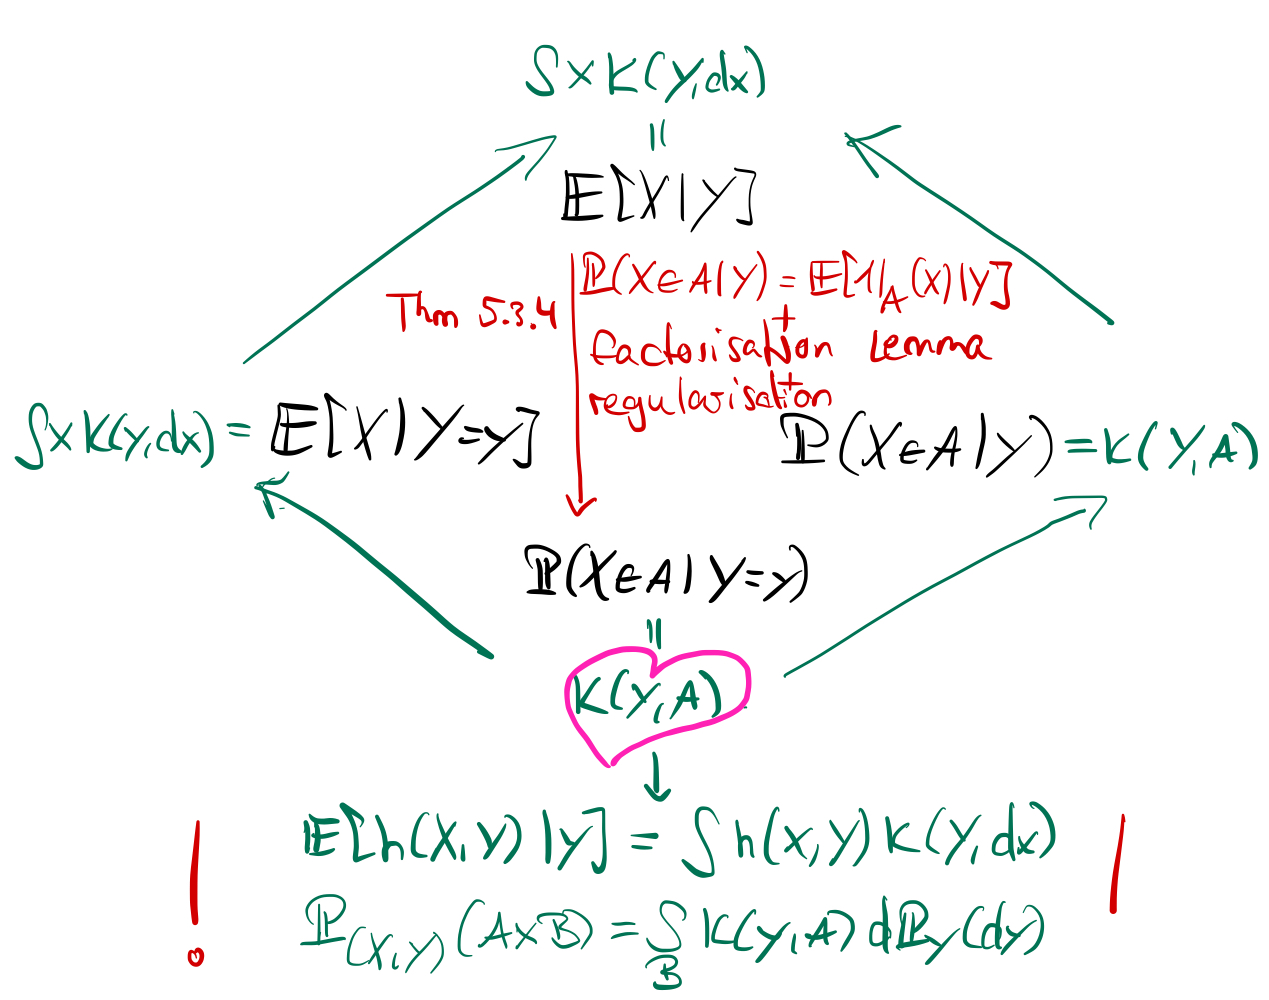
\includegraphics[scale=0.19]{CE9.jpeg}		
%	\end{center}
%		\vspace{-0.3cm}
%	\caption*{The logic behind the disintegration kernel and conditional expectation}
%\end{figure}

\begin{figure}[h]
\begin{center}
\begin{tikzpicture}[scale=0.8,transform shape]
  \tikzmath{\x = 3.3;}
  \node[darkgreen] (E1) at (0,\x) {$\int_{\mathbb{R}} x \kappa(Y,dx)$} ;
  \node[darkgreen,rotate=90,scale=0.7] (eq1) at ($(E1.south)+(0,-0.2)$) {}; 
  \node[darkgreen,rotate=90,scale=0.7] (eq) at ($(E1.south)+(-0.12,-0.2)$) {$=$}; 
  \node[black,scale=0.7] (equation1) at ($(eq1.south) +(-0.2,-0.4)$) {$\mathbb{E}[X|Y]$};

  \node[darkgreen] (E2) at (\x,0) {$\kappa(Y,A)$} ;
  \node[darkgreen,scale=0.7] (eq2) at ($(E2.west)+(0,-.02)$) {$=$}; 
  \node[black,scale=0.7] (equation2) at ($(eq2.west) +(-0.6,0)$) {$\mathbb{P}(X \in A|Y)$};

  \node[darkgreen] (E3) at (0,-\x) {$ \kappa(y,A)$} ;
  \node[darkgreen,rotate=90,scale=0.7] (eq3) at ($(E3.north)+(0,0.2)$) {$=$}; 
  \node[black,scale=0.6] (equation3) at ($(eq3.south) +(-0.2,0.4)$) {$\mathbb{P}(X \in A | Y=y)$};

  \node[darkgreen] (E4) at (-\x,0) {$\int_{\mathbb{R}}x \kappa(y,dx)$} ;
  \node[darkgreen,scale=0.7] (eq4) at ($(E4.east)+(0,-.02)$) {$=$}; 
  \node[black,scale=0.7] (equation4) at ($(eq4.east) +(0.6,0)$) {$\mathbb{E}[X|Y=y]$};

  \draw[-stealth,draw=darkgreen] (E4)--(E1);
  \draw[-stealth,draw=darkgreen] (E2)--(E1);
  \draw[-stealth,draw=darkgreen] (E3)--(E2);
  \draw[-stealth,draw=darkgreen] (E3)--(E4);
  
  \draw[-stealth,draw=red] (equation1) -- (equation3);
  \node[red,scale=0.6] (theorem1) at ($(eq1.south) +(-1.,-1.8)$) {};
  \node[red,scale=0.5] (theoremEq) at ($(theorem1.east) +(1.9,-0)$) {$\mathbb{P}(X\in A | Y) = \mathbb{E}[\mathbbm{1}_A(x)|Y]$};
  \node[red,scale=0.5] (theoremTxt1) at ($(theoremEq.south)+(-0.25,-0.2)$) {factorisation lemma};
  \node[red,scale=0.5] (theoremTxt2) at ($(theoremTxt1.south) +(-0.18,-0.1)$) {+ regularisation};

  \draw[-stealth,draw=darkgreen] (E3) -- (0,-4);
  \node[darkgreen,scale=0.7] (equation5) at (0.2,-4.3) {$\mathbb{E}[h(X,Y)|Y] = \int h(x,y)\ k(y,dx)$};
  \node[darkgreen,scale=0.7] (equation6) at (0.26,-4.8) {$\mathbb{P}_{(x,y)}(A\times B) = \int_B k(y,A)\mathbb{P}_y(dy)$};
  \node[red,scale=2] (!) at (-1.9,-4.5)  {!}; 
  \node[red,scale=2] (!) at (2.4,-4.5)  {!}; 
\end{tikzpicture}
	\caption*{The logic behind the disintegration kernel and conditional expectation}
\end{center}
\end{figure}
We finish the section with a discussion on conditioning on zero sets.	A bit of care is needed about the interpretation of $\P(X\in A|Y=y)$ as typically the event $\{Y=y\}$ has probability zero. One can easily get confused about the notation as the elementary conditional probability $\P(A|B)=\frac{\P(A\cap B)}{\P(B)}$ is not defined for null-sets $B$. The point is that we did not use the elementary definition of conditional probability. Instead, we constructed in some obscure way a mapping $y\mapsto \P(X\in A|Y=y)$ that satisfies a general total probability rule 
	\begin{align*}
			\P(X\in A)=\int_\R \P(X\in A|Y=y)\, \P_Y(\mathrm d y),\quad A\in \mathcal B(\R).
	\end{align*}
	In general there is no reason to expect any relation to elementary conditioned probabilities. Nonetheless, there are two situation in which the definition $\P(X\in A|Y=y)=\kappa(y,A)$ coincides with elementary conditioning and that's why we abuse the notation of conditional probability.\smallskip
	
		 If $Y$ is discrete, then the above formulas give
			\begin{align*}
				\P(X\in A|Y=y)=\begin{cases} 
								\P(X\in A|Y=a_k) &: y=a_k\\
								0&:\text{otherwise}
							\end{cases}
			\end{align*}
		with elementary conditional probability on the right hand side.\smallskip			
			
		 If $X$ and $Y$ are jointly absolutely continuous with density $f>0$ there is another way to define $\P(X\in A|Y=y)$ through a limiting procedure. The result is exactly the same:
			\begin{align*}
	\P(X\in A|Y=y)&:=\lim_{\varepsilon \to 0}\P(X\in A|Y\in (y-\varepsilon,y+\varepsilon))\\
	&=\lim_{\varepsilon\to 0} \frac{\int_{y-\varepsilon}^{y+\varepsilon} \int_A f(x,y)\dint x\,dy }{\int_{y-\varepsilon}^{y+\varepsilon} f_y(y)\dint x}\\
	\overset{\text{l'Hospital}}&{=} \frac{\int_A f(x,y)\dint x}{f_y(y)}=\kappa(y,A),
\end{align*}
with the kernel for absolutely continuous random vectors.




\section{General regular conditional distributions}
	\marginpar{\textcolor{red}{Not part of\\ the course}}

We finish the discussion of conditional expectation with a generalisation of Theorem \ref{formeln} towards conditional expectations on a general $\sigma$-algebra $\mathcal F$. We want to provide a computation rule
\begin{align}\label{integrall}
	\E[h(X)|\mathcal F]=\int_\R h(x) \,\P(X\in \dint x|\mathcal F)\quad \text{a.s.}
\end{align}	
 for all measurable $h$. For $\mathcal F=\sigma(Y)$ we proved such a formula using the "{}random"{} measures $\P(X\in \mathrm d x|Y)=\kappa(Y,\mathrm dx)$. The general setting does not provide a kernel $\P(X\in A|Y=y)=\kappa(y,A)$ to work with but still allows us to construct a "{}random"{} measure  satisfying \eqref{integrall}
 
% 
 %The answer is yes, but this is far from obvious. Let's try to see where the problems come from by looking at classical expectations. Suppose we know $\E[h(X)]$ for enough measurable functions, say all indicators. Then we could recover the law of $X$ on $\mathcal B(\R)$ via $\P_X(B)=\P(X\in B)=\E[\mathbf 1_B(X)]$ and from this derive the formula $\E[h(X)]=\int_\R h(x) \P_X(\dint x)$ via monotone convergence. Suppose we did the same for the conditional expectation and define $\P_{X|\mathcal F}(B):=\E[\mathbf 1_B(X)|\mathcal F]$. Note that those are random variables! Immediately we will run into trouble. The problem is that all those conditional expectations $\E[\mathbf 1_B(X)|\mathcal F]$ are only defined up to nullsets. Since we have uncountably many Borel-sets the (random) measure $B\mapsto \P_{X|\mathcal F}(B)$ would be defined only up to an uncountable union of nullsets and this could be anything. We can work our way around this by choosing versions of the conditional expectation which are all defined on the same probability space. For this we will use the separability of $\R$, i.e. with $\Q$ there is a countable dense subset, so that we only need to define the measure on intervals with rational boundary. Since countable unions of nullsets are nullsets,
%	\begin{align*}
%		0 \leq \mu \left( \bigcup\limits_{k=1}^{\infty}N_k \right) \leq \sum \limits_{k=1}^{\infty} \mu (N_k) = \sum \limits_{k=1}^{\infty} 0 = 0,
%	\end{align*}
%	no problem will occur. If we can carry this out we will call this (random) measures $(\omega, B)\mapsto \P_{X|\mathcal F}(B)(\omega)$ the conditional distribution of $X$ given $\mathcal F$. To do anything interesting (like integration) with such measures we should also find a version which is measurable in $\omega$. If we can achieve this we will speak of a regular conditional distribution of $X$ given $\mathcal F$. \smallskip
		
%	As objects of that kind appear in many fields of probability we should give it a name:
\begin{ldef}
\begin{deff}
	Suppose $(\Omega, \mathcal A, \P)$ is a probability space. A Markov kernel $\mu$ on $\Omega\times \mathcal B(\R)$ is called a \textbf{random measure}.
\end{deff}
\end{ldef}
The simplest example of a random measure already appeared in the previous section. If $\kappa$ is a kernel and $Y$ is a random variable, then $\kappa(Y,\cdot)$ is a random measure. The measure property is clear, the measurability follows as the concatenation of $Y$ and $\kappa$ is measurable again.\smallskip

Random measures can be found at very different places in statistics and probability theory under different names. For conditional expectations we use random measures to define regular conditional distributions:
\begin{ldef}
\begin{deff}\label{def_regular_cond_expectation}
%	\begin{enumerate}[label=(\roman*)]
%		\item 
Let $X$ be an integrable random variable on $(\Omega,\cA,\mathbb{P})$ and $\cF \subseteq \cA$ a sub-$\sigma$-algebra. A random measure $\mu$ on $\Omega\times \cB(\mathbb{R})$ is called a regular version of the conditional distribution (or a \textbf{regular conditional distribution}) of X given {$\cF$} if \[ \mu(\omega,B)=\mathbb{E}\big[\mathbf 1_B(X)\big|  \cF\big](\omega)\quad \text{a.s.} \]
		for all $B \in \cB(\mathbb{R})$. We will write $\P(X\in B|\mathcal F)(\omega)$, $\P_{X|\mathcal F}(B)(\omega)$, or $\mathbb{E}[\mathbf 1_B(X)\big|  \cF](\omega)$ instead of $\mu(\omega,B)$ but often skip the dependence of $\omega$ just as we usually do for random variables.
\end{deff}
\end{ldef}
Going back again to the special case $\mathcal F=\sigma(Y)$ from the previous section, we obtain our first example. Theorem \ref{formeln} showed that 
\begin{align*}
	\E[\mathbf 1_B(X)|Y]=\kappa(Y,B)\overset{\text{Notation}}=\P(X\in  B|Y),
\end{align*}
which is exactly the formula we want to generalise for $\mathcal F$.\smallskip

Let us now prove the existence of a regular conditional expectation for general $\sigma$-algebras:
\begin{lsatz}
\begin{theorem}\label{existence_regular_dist}
%	\begin{enumerate}[label=(\roman*)]
	%		\item 
	If X is an integrable random variable on  $(\Omega,\cA,\mathbb{P})$ and $\cF \subseteq  \cA$ is a sub-$\sigma$-algebra, then there exists a regular conditional distribution $\mu$ of $X$ given $\cF$.
%			\item If $X$,$Y$ are random variables on $(\Omega , \cA , \mathbb{P})$, then the regular conditional distribution of $X$ given $Y$ exists.
%	\end{enumerate}		
\end{theorem}
\end{lsatz}



\begin{proof}[Proof]
%	\begin{enumerate}[label=(\roman*)]
%		\item
Our strategy is as follows:
			\begin{itemize}
				\item[(i)] Define a candidate measure $\mu(\omega,\cdot)$.
				\item[(ii)] Check that $\mu$ is a random measure on $\Omega \times \mathcal B(\R)$.
				\item[(iii)] Check for all $B\in \mathcal B(\R)$ that $\mu(\cdot,B)$ is a version of $\E[\mathbf 1_{B}(X)|\mathcal F]$.
			\end{itemize}
			\textbf{Step (i):} The main idea of the argument is that measures on $\mathcal B(\R)$ are uniquely determined by their commulative distribution function (Dynkin-Systems + Carath\'eodory, see Theorem \ref{EindVert}). For fixed $t\in\Q$ define the $\mathcal F$-measurable random variable
			\[ F_\omega(t):= \mathbb{E}\big[\mathbf 1_{(-\infty , t]}(X) | \cF\big](\omega) \]
			as an arbitrary version of the conditional expectation which exists by Theorem \ref{existenceCE}. Using monotonicity of conditional expectations and the countability of $\Q$, there is a measurable set $\cM^1\in \mathcal A$ with $\mathcal P(\mathcal M^1)=1$ so that 
			\begin{align*}
				t\mapsto F_\omega(t) \quad\text{ is increasing on $\Q$ for all }\omega \in \mathcal M^1.
			\end{align*}
			The set $\mathcal M^1$ is the intersection of the countably many sets $\mathcal M_{t,s}$ of measure $1$ on which Theorem \ref{cond_properties} (iii) gives $F_\omega(s)\leq F_\omega(t)$ for $s<t$. Using dominated convergence for conditional expectations (Theorem \ref{cond_properties} (ix)) we find another measurable set $\mathcal M^2$ with $\P(\mathcal M^2)=1$ so that
			\begin{align*}
				\lim_{t\to+\infty, t\in \Q} F_\omega(t)=1\quad \text{and}\quad 	\lim_{t\to-\infty, t\in \Q} F_\omega(t)=0\quad\text{ for all }\omega\in \mathcal M^2.
			\end{align*}
			Also with dominated convergence we find another measurable set $\mathcal M^3$ with $\P(\mathcal M^3)=1$ so that right-continuity holds on $\Q$:
			\begin{align*}
				\lim_{t\downarrow s, t\in \Q} F_\omega(t)=F_\omega(s) \quad \text{ for all } s \in \Q\text{ and }\omega \in \mathcal M^3.
			\end{align*}			
			If now we fix some arbitrary distribution function $\tilde F$ and define $F_\omega(t):=\tilde F(t)$ for $\omega \notin \mathcal M^3$, then we have defined $F_\omega(t)$ for all $t\in\Q$ and all $\omega \in \Omega$ such that $t\mapsto F_\omega(t)$ satisfies the properties of distribution functions on $\Q$ for all $\omega\in \Omega$ and $F_\cdot (t)$ is a version of $\E[\mathbf 1_{(-\infty,t]}(X)|\mathcal F]$ for all $t\in \Q$.\smallskip
			
			Now we extend $\Q$ to $\R$ by defining
			\begin{align*}
				 \overline{F}_\omega(s):= \inf \big\{ F_\omega(t) \big| t > s \, , \, t \in \mathbb{Q} \big\},\quad s\in \mathbb{R}, \omega \in \Omega.
			\end{align*}
			It is a bit tedious (basic analysis) to show that $t\mapsto \overline F_\omega(t)$ inherits the properties of a distribution function from $F_\omega$. Hence, by Theorem \ref{EindVert} there are probability measures $\mu(\omega,\cdot)$ on $\mathcal B(\R)$ for all $\omega\in \Omega$.\smallskip
			
			\textbf{Steps (ii) and (iii):} We use our favorite argument of "{}good sets"{} from measure theory (compare the proof of Theorem \ref{Dynkin-Folgerung}). Let
			\begin{align*}
				\mathcal B=\{ A\in \mathcal A: \mu(\cdot, A)\text{ is a version of }\E[\mathbf 1_{A}(X)|\mathcal F]\text{ and }\omega \mapsto \mu(\omega, A)\text{ is a random measure}\}.
			\end{align*}
			We have to prove that $B=\mathcal B(\R)$ is a Dynkin-system and contains an $\cap$-stable generator of $\mathcal B(\R)$. This works essentially as in the proof of Theorem \ref{kernel}.
%			\begin{itemize}
%				\item The Dynkin-system property follows from the properties of conditional expectation. Recall the definition of a Dynkin-system now!
%				\item $\mathcal E:=\{(-\infty,t]:t\in\R\}$ is a $\cap$-stable generator of $\mathcal B(\R)$ and contained in $\mathcal B$ through the construction of $\mu$.
%			\end{itemize}
			
			
			
%			\begin{itemize}
%				\item $\omega \mapsto \mu(\omega,(-\infty,t\,]) = F(t,\omega)\mathds 1_{\cR}(\omega) + \mathds 1_{[\, 0\, , \, \infty\, )}(t)\mathds 1_{\cR^C}(\omega) $ is $\cF$-measurable because all parts of on the right hand side are measurable.
%				\item $\omega \mapsto \mu(\omega,B)$ is a measure by definition.
%				\item For $\cA \subseteq \cF$ we have by definition $\forall t\in \mathbb{R}$:
%					\begin{align*}
%						 \mathds E\big[\mathds 1_A \mu\big(\cdot,\, (\, -\infty\, , \, t \, ]\big)\big] \overset{\text{Def.}}&{=} \mathds E\big[\mathds 1_A \mathbb{P}\big(X \in (\, -\infty\, , \, t \, ]\, | \, \cF\big)\big] \\
%						 \overset{\cA \subseteq \cF}&{=} \mathds E\big[\mathds 1_A \mathds 1_{(\, -\infty\, , \, t \, ]}(X)\big]
%					\end{align*}
%					Uniqueness theorem for measures shows \[ \mathds E \big[ \mathds 1_A \mu (\cdot,B)\big] = \mathds E\big[ \mathds 1_A \mathds 1_B(X) \big] ,\] hence, \[ \mu(\cdot,B)= \mathds E \big[ \mathds 1_B(X)\, \big| \, \cF \big] \overset{\text{Def.}}{=} \mathbb{P}\big(X\in B \, \big| \, \cF\big) \:\:\:\: \mathbb{P}\text{-a.s.} \]
%			\end{itemize}r
\end{proof}
We can now come back to the motivation and compute different conditional expectations just the way we are used to for the classical expectation:
\begin{lsatz}
\begin{prop}
	Suppose $h:\mathbb{R}\mapsto\mathbb{R}$ is Borel-measurable such that $h(X)\in \mathcal L^1(\Omega, \mathcal A, \P)$, then
%	\begin{enumerate}[label=(\roman*)]
%		\item
 \begin{align*}
 	\mathds E[ h(X) |  \cF] =  \int_{\mathbb{R}} h(x)\,\P_{X|\mathcal F}(\mathrm dx)\quad\text{a.s.}
\end{align*}
%		\item $\mathds E[ h(X)\, | \, Y=y ] = \int_{\mathbb{R}}h(x)\mathbb{P}_{X|Y=y}(\dint x)$
%	\end{enumerate}
\end{prop}
\end{lsatz}

\begin{proof}[Proof]
	If $f=\mathbf 1_B$, $B\in \mathcal B(\R)$, the statement follows from the definition of $\P_{X|\mathcal F}$. Now let $h\geq 0$ measurable and $h_n = \sum\limits_{k=1}^{n}\alpha_k\mathds 1_{B_k}$ a sequence of simple functions with $h_n \uparrow h$. Then, for $A\in\cF$,
			\begin{align*}
				\mathds E\big[\mathds 1_A h(X)\big] \overset{\text{MCT}}&{=} \lim\limits_{n\rightarrow \infty}\mathds E\big[\mathds 1_A h_n(X)\big] \\
																		\overset{\text{lin.}}&{=} \lim\limits_{n\rightarrow \infty} \sum\limits_{k=1}^{n}\alpha_k \mathds E\big[ \mathds 1_A \mathds 1_{B_k}(X)\big] \\
																		\overset{A\in \mathcal F}&{=} \lim\limits_{n\rightarrow \infty} \sum\limits_{k=1}^{n} \alpha_k \mathds E\big[ \mathds 1_A \mathds E[ \mathds 1_{B_k}(X)\, | \, \cF] \big] \\
																		&= \lim\limits_{n\rightarrow \infty} \sum\limits_{k=1}^{n}\alpha_k \mathds E\big[ \mathds 1_A  \P_{X|\mathcal F}(B_k)\big] \\
																		\overset{\text{lin.}}&{=} \lim\limits_{n\rightarrow\infty} \mathds E\Big[ \mathds 1_A \sum\limits_{k=1}^{n}\alpha_k \P_{X|\mathcal F}(B_k)\Big] \\
																		&= \lim\limits_{n \rightarrow \infty} \mathds E \Big[ \mathds 1_A \int_{\R} h_n(x)]P_{X|\mathcal F}(\mathrm dx)\Big] \\
																		\overset{\text{2x MCT}}&{=} \mathds E \Big[ \mathds 1_A \int_{\R} h(x)\P_{X|\mathcal F}(\mathrm dx)\Big].
			\end{align*}
			This proves the expectation property of conditional expectation. With the same approximation we also obtain the measurability property as $\int_{\R} h(x)\mu(\cdot,\mathrm d x)$ is a pointwise limit of $ \sum\limits_{k=1}^{n}\alpha_k P_{X|\mathcal F}(B_k)$ which are all $\mathcal F$-measurable. Hence, the right-hand side satisfies both defining properties of $\mathbb E[\big[ h(X)|\mathcal F\big]$ and as such is a version of the conditional expectation. For general $h$ we write $h=h^+-h^-$ and use linearity as usual.
\end{proof}

%\vspace{-2mm}
%	\begin{figure}[h]
%	\begin{center}
%		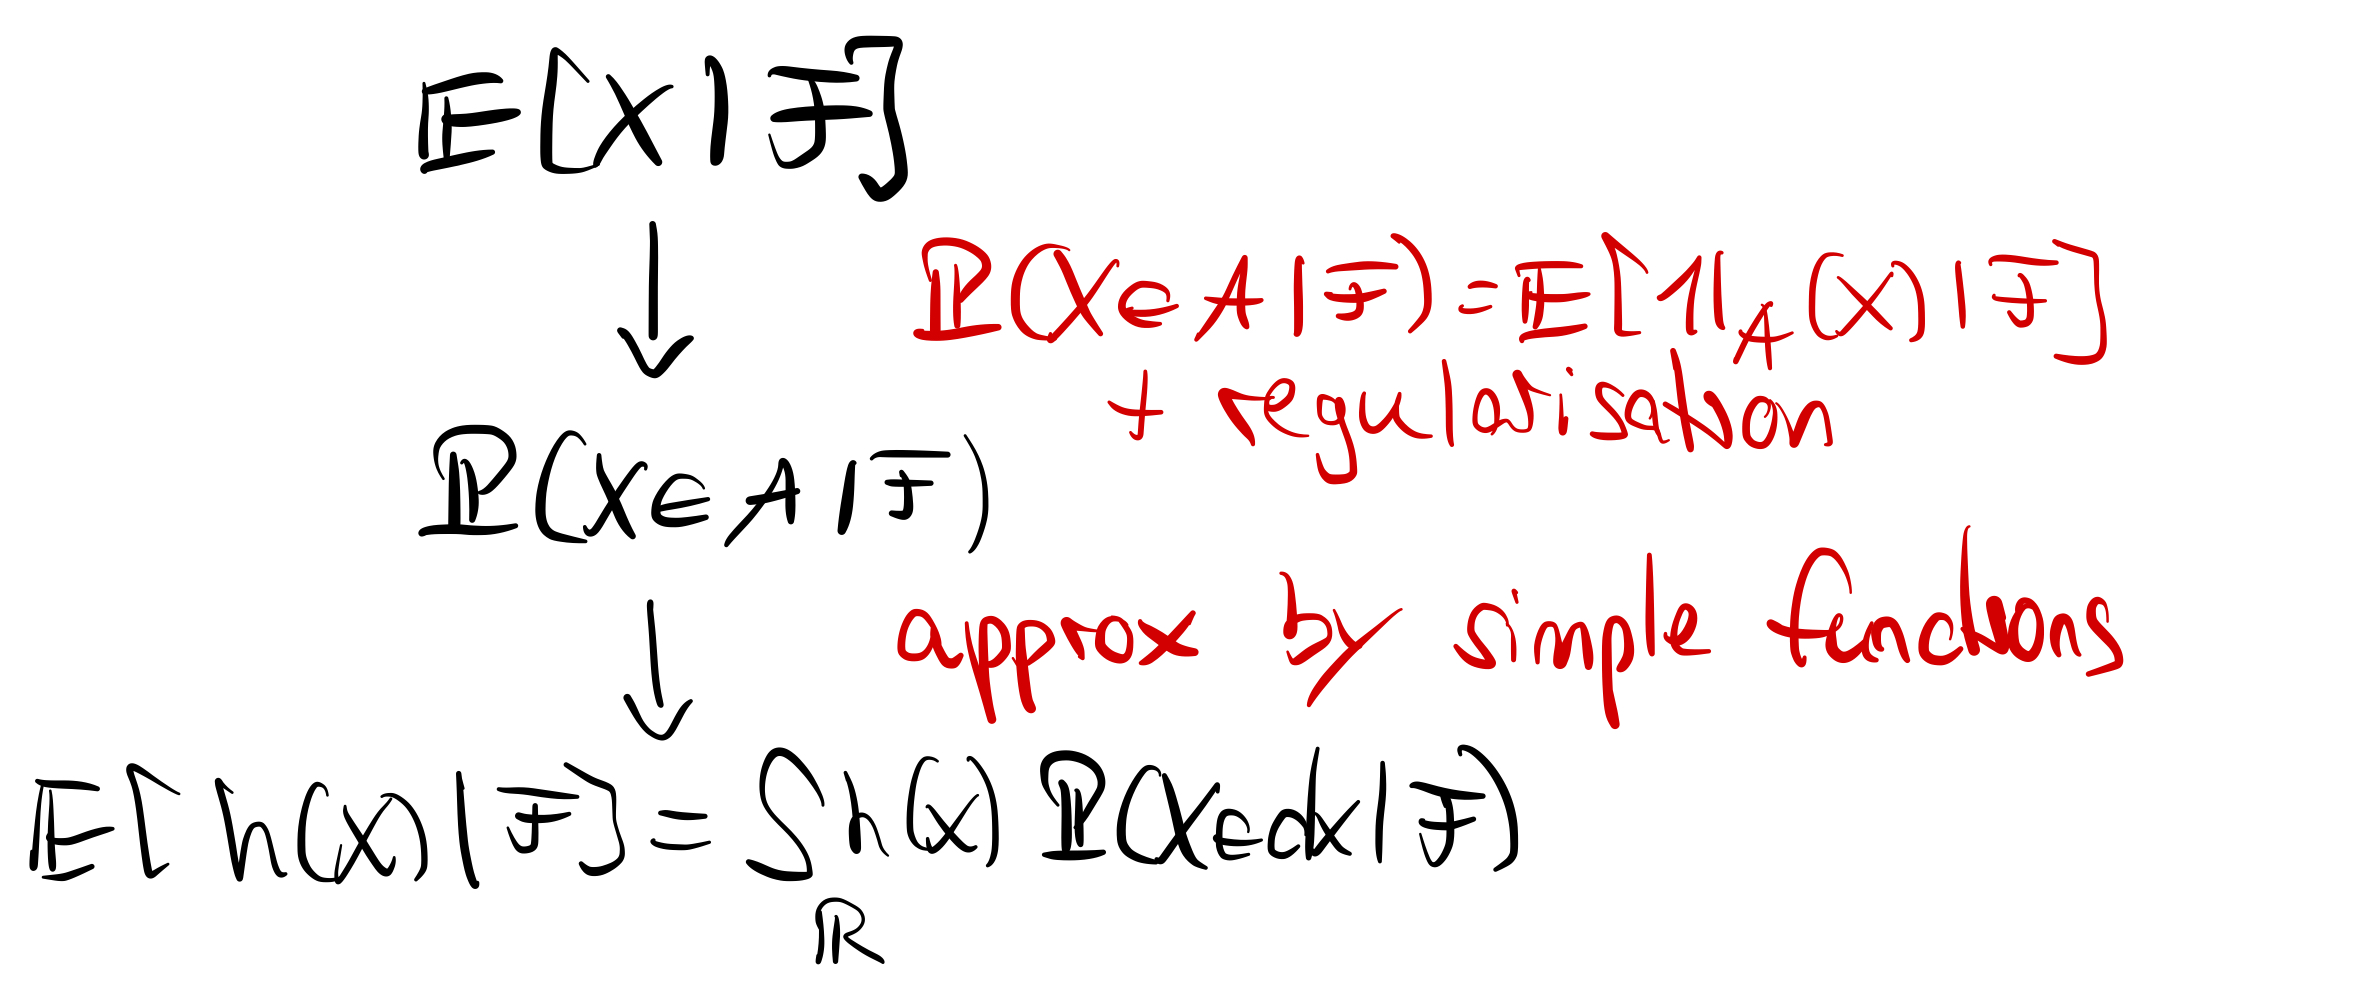
\includegraphics[scale=0.1]{CE10.jpeg}		
%	\end{center}
%		\vspace{-0.3cm}
%	\caption*{The logic behind the regular conditional probability}
%\end{figure}

\begin{figure}[h]
\begin{center}
\begin{tikzpicture}[scale=.9,transform shape]
  \node[black,scale=1] (equation1) at (0,0) {$\mathbb{E}[X|\mathcal{F}]$};
  \node[black,scale=1] (equation2) at (0,-2) {$\mathbb{P}(X \in A |\mathcal{F})$};
  \node[black,scale=1] (equation3) at (0,-4) {$\mathbb{E}[h(X)|\mathcal{F}] = \int_{\mathbb{R}} h(x) \mathbb{P}(X \in dx |\mathcal{F})$};
  
  \node[red,scale=1] (txt1) at (2.2,-0.8) {$\mathbb{P}(X \in A |\mathcal{F}) = \mathbb{E}[\mathbbm{1}_A(X) |\mathcal{F}]$};
  \node[red,scale=1] (txt2) at ($(txt1.south) + (-0.85,0)$) {+ regularisation};
  \draw[-stealth,black] (equation1) -- (equation2);
  \node[red,scale=1] (txt2) at (2.6,-2.8) {approximate by simple functions};
  \draw[-stealth,black] (equation2) -- (equation3);
\end{tikzpicture}
  \caption*{The logic behind the regular conditional probability}
\end{center}
\end{figure}


%In virtue of computations performed for classical expectations we can go one step further and also as for conditional densities that allow to compute the random measure $\P_{X|\mathcal F}$ through integrals over random densities.
%\begin{deff}
%	A mapping $f_{X|\mathcal F}:\Omega\times \R\to \R$ is called conditional density of $X$ given $\mathcal F$ if 
%	\begin{itemize}
%		\item $x\mapsto f_{X|\mathcal F}(\omega, x)$ is Borel-measurable for all $\omega\in \Omega$,
%		\item $\omega\mapsto f_{X|\mathcal F}(\omega,x)$ is $\mathcal A$-measurable for all $x\in \R$,
%		\item $\P_{X|\mathcal F}(B)(\omega)=\int_B f_{X|\mathcal F}(\omega,x)\dint x$ a.s. for all $B\in \mathcal B(\R)$.
%	\end{itemize}
%\end{deff}
%Such measurability conditions are certainly frightening on first view. Just keep in mind that all integrals that we possible consider need measurability for the definition. Hence, whenever we see mappings in probability theory we will need measurability. As an example let us come back to the case of jointly absolutely continuous random variables from Proposition \ref{pjc}:
\begin{lwarnhinweis}
As soon as you attend a lecture on general Markov processes, the object of regular conditional expectation will be central to define the Markov property as
\begin{align*}
	\P(X_{t+s}\in A| \mathcal F_t)=\P(X_{t+s}\in A|X_t)\quad\text{a.s.},
\end{align*}
where $\mathcal F_t=\sigma(X_s:s\leq t)$ is the information of the process up to time $t$. This is a way of formalising the idea of the future distribution given the past is equal to the future distribution given the entire past.
\end{lwarnhinweis}

It is typically a good exercise to check Markov inequalities as the proofs require the standard tools of probability theory. Do it!
\begin{luebung}
Let $h:[0,\infty)\to [0,\infty)$ increasing, then
\begin{align*}
	\P(|X|>\epsilon|\mathcal F)\leq \frac{\E[h(X)|\mathcal F]}{h(\epsilon)}\quad \text{a.s.}
\end{align*}
\end{luebung}



%\begin{proof}
%	Define $\nu(y,B) = \int_{B} f_{X|Y}(x,y)\dint x$ and show the defining property for $\nu(Y,B)$: Let $g$ be $\sigma(Y)$-measurable:
%	\begin{align*}
%		\mathds E\big[g(Y)\nu(Y,B)\big]&= \int_{\Omega} g \big( Y(\omega)\big)\nu\big(Y(\omega),B\big)\dint\mathbb{P}(\omega) \\
%								&= \int_{\Omega} g\big(Y(\omega)\big) \int_{B} f_{X|Y}\big(x,Y(\omega)\big)\dint x \dint \mathbb{P}(\omega) \\
%								\overset{\text{no problem, why?}}&{=} \int_{\Omega} \frac{g\big(Y(\omega)\big)}{f_y\big(Y(\omega)\big)} \int_{B}f\big(x,Y(\omega)\big)\dint x \dint \mathbb{P}(\omega)\\
%								&= \int_{\mathbb{R}}\frac{g(Y)}{f_y(y)} \int_{B} f(x,y)\dint x f_y(y)\dint y  \\
%								&= \int_{\mathbb{R}} \int_{\mathbb{R}} g(y)\mathds 1_B(x)f(x,y)\dint x \dint y \\
%								&= \mathds E\big[g(Y)\mathds 1_B(X)\big]
%	\end{align*}
%\end{proof}

